% **************************************************************************************************************
% A Classic Thesis Style
% An Homage to The Elements of Typographic Style
%
% Copyright (C) 2012 Andr\'e Miede http://www.miede.de
%
% If you like the style then I would appreciate a postcard. My address 
% can be found in the file ClassicThesis.pdf. A collection of the 
% postcards I received so far is available online at 
% http://postcards.miede.de
%
% License:
% This program is free software; you can redistribute it and/or modify
% it under the terms of the GNU General Public License as published by
% the Free Software Foundation; either version 2 of the License, or
% (at your option) any later version.
%
% This program is distributed in the hope that it will be useful,
% but WITHOUT ANY WARRANTY; without even the implied warranty of
% MERCHANTABILITY or FITNESS FOR A PARTICULAR PURPOSE.  See the
% GNU General Public License for more details.
%
% You should have received a copy of the GNU General Public License
% along with this program; see the file COPYING.  If not, write to
% the Free Software Foundation, Inc., 59 Temple Place - Suite 330,
% Boston, MA 02111-1307, USA.
%
% **************************************************************************************************************
% Note:
%    * You must not use "u etc. in strings/commands that will be spaced out (use \"u or real umlauts instead)
%    * New enumeration (small caps): \begin{aenumerate} \end{aenumerate}
%    * For margin notes: \marginpar or \graffito{}
%    * Do not use bold fonts in this style, it is designed around them
%    * Use tables as in the examples
%    * See classicthesis-preamble.sty for useful commands
% **************************************************************************************************************
% To Do:
%   * [high] Check this out: http://www.golatex.de/koma-script-warnung-in-verbindung-mit-listings-package-t2058.html
%   * [medium] mathbb in section-titles/chapter-titles => disappears somehow in headlines!!!
% **************************************************************************************************************
\documentclass[ twoside,openright,titlepage,numbers=noenddot,headinclude,%1headlines,% letterpaper a4paper
                footinclude=true,cleardoublepage=plain,abstractoff, % <--- obsolete, remove (todo)
                BCOR=5mm,paper=a4,fontsize=11pt,%11pt,a4paper,%
                portuguese,
                dottedtoc, % adicionar pontinhos na lista de conteúdos
                ]{scrreprt}


% UTF-8 support with latin9 (ISO-8859-9) = latin1+"Euro sign"
\PassOptionsToPackage{utf8}{inputenc}   
\usepackage{inputenc}  
 
% ****************************************************************************************************
% Personal data and user ad-hoc commands
% ****************************************************************************************************
\newcommand{\myTitle}{O que é que as redes convolucionais conseguem aprender \xspace}
\newcommand{\myDegree}{Licenciatura em Eng.ª Informática\xspace}
\newcommand{\myNameOne}{Estudante Frederico Assunção de Sá Bento\xspace}
\newcommand{\myNumberOne}{2211012}
\newcommand{\myNameTwo}{Estudante Pedro Nuno Tempero Serafim\xspace}
\newcommand{\myNumberTwo}{2211084}


\newcommand{\myProfOne}{Professor Doutor Carlos Fernando de Almeida Grilo
\href{mailto:luis.conde@ipleiria.pt}{(carlos.grilo@ipleiria.pt)}\xspace}
\newcommand{\myProfTwo}{Professor Doutor José Carlos Bregieiro Ribeiro  \href{mailto:hugo.costelha@ipleiria.pt}{(jose.ribeiro@ipleiria.pt)}\xspace}
\newcommand{\myProfThree}{Professor Doutor Rolando Lúcio Germano Miragaia
\href{mailto:catarina.reis@ipleiria.pt}{(rolando.miragaia@ipleiria.pt)}\xspace}
% \newcommand{\myProfTwo}{Professor Doutor XXXX XXXXX XXXXX \href{mailto:xxxxxx@ipleiria.pt}{(xxxxxx@ipleiria.pt)}\xspace}

\newcommand{\myFaculty}{Politécnico de Leiria\xspace}
\newcommand{\mySchool}{Escola Superior de Tecnologia e Gestão\xspace}
\newcommand{\myDepartment}{Departamento de Engenharia Informática\xspace}
\newcommand{\myLocation}{Leiria\xspace}

\newcommand{\myTime}{Março de 2024\xspace}
\newcommand{\mySchoolYear}{2023 -- 2024\xspace}
\newcommand{\myVersion}{versão 0.1\xspace}            
                
                
%*******************************************************
% Note: Make all your adjustments in here
%*******************************************************
% ****************************************************************************************************
% classicthesis-config.tex 
% formerly known as loadpackages.sty, classicthesis-ldpkg.sty, and classicthesis-preamble.sty 
% Use it at the beginning of your ClassicThesis.tex, or as a LaTeX Preamble 
% in your ClassicThesis.{tex,lyx} with \input{classicthesis-config}
% ****************************************************************************************************  
% If you like the classicthesis, then I would appreciate a postcard. 
% My address can be found in the file ClassicThesis.pdf. A collection 
% of the postcards I received so far is available online at 
% http://postcards.miede.de
% ****************************************************************************************************

% ****************************************************************************************************
% 1. Configure classicthesis for your needs here, e.g., remove "drafting" below 
% in order to deactivate the time-stamp on the pages
% ****************************************************************************************************
\PassOptionsToPackage{
                    eulerchapternumbers,
                    drafting, % comentar para remover a linha com a versão
                    pdfspacing,
                    %floatperchapter,
                    %linedheaders,%
                    subfig,beramono,
                    eulermath,
                    parts
                    }{classicthesis}
% Available options for classicthesis.sty 
% (see ClassicThesis.pdf for more information):
% drafting
% parts nochapters linedheaders
% eulerchapternumbers beramono eulermath pdfspacing minionprospacing
% tocaligned dottedtoc manychapters
% listings floatperchapter subfig
% ********************************************************************

% ********************************************************************
% Triggers for this config
% ******************************************************************** 
\usepackage{ifthen}
\newboolean{enable-backrefs} % enable backrefs in the bibliography
\setboolean{enable-backrefs}{false} % true false

% ****************************************************************************************************


% ********************************************************************
% Setup, finetuning, and useful commands
% ********************************************************************
\newcounter{dummy} % necessary for correct hyperlinks (to index, bib, etc.)
\newlength{\abcd} % for ab..z string length calculation
\providecommand{\mLyX}{L\kern-.1667em\lower.25em\hbox{Y}\kern-.125emX\@}
\newcommand{\ie}{\textit{i.\,e.}\xspace}
\newcommand{\Ie}{\textit{I.\,e.}\xspace}
\newcommand{\eg}{\textit{e.\,g.}\xspace}
\newcommand{\Eg}{\textit{E.\,g.}\xspace} 
\newcommand{\etc}{\textit{etc}\xspace} 


% ****************************************************************************************************
% \DeclareTextFontCommand{\code}{\fontfamily{pcr}\scriptsize}


% ****************************************************************************************************
% 3. Loading some handy packages
% ****************************************************************************************************
% ******************************************************************** 
% Packages with options that might require adjustments
% ******************************************************************** 

\PassOptionsToPackage{portuguese}{babel}
\usepackage{babel}

 
%%%%%%%%%%%%%%%%%%%%%%%%%%%%%%%%%%%%%%%%%%%%%%%%%%%%%
% Bibliografia
%%%%%%%%%%%%%%%%%%%%%%%%%%%%%%%%%%%%%%%%%%%%%%%%%%%%%
% package recomendada para usar com o biblatex
\usepackage{csquotes}

% carrega a package biblatex
\usepackage[
    backend=biber,    % usar o biber para processar
    style=authoryear, % estilo de citação
    sortcites=true,
    maxcitenames=2,   % a partir de 2 escreve "et al."
]{biblatex} 

% para adicionar uma vírgula antes do ano: (Dirac, 1981)
\renewcommand*{\nameyeardelim}{\addcomma\space}

%  dica: configurar o kile para reconhecer os comandos:
%    \parencite{bibkey}
%    \textcite{bibkey}
%    \citeauthor{bibkey}
%    \citetitle{bibkey}
%    
%    Settingis -> Configure Kile -> Latex/General -> Commands/Configure -> Commands/Citation -> add
%%%%%%%%%%%%%%%%%%%%%%%%%%%%%%%%%%%%%%%%%%%%%%%%%%%%%
 
\usepackage{float}

\PassOptionsToPackage{fleqn}{amsmath}		% math environments and more by the AMS 
\usepackage{amsmath}

\usepackage{multirow}
 
%******************************************************************** 
% General useful packages
%******************************************************************** 
\PassOptionsToPackage{T1}{fontenc} % T2A for cyrillics
\usepackage{fontenc}

\usepackage{textcomp} % fix warning with missing font shapes
\usepackage{scrhack} % fix warnings when using KOMA with listings package          
\usepackage{xspace} % to get the spacing after macros right  
\usepackage{mparhack} % get marginpar right
% \usepackage{fixltx2e} % fixes some LaTeX stuff 

\PassOptionsToPackage{printonlyused,smaller}{acronym}
\usepackage{acronym} % nice macros for handling all acronyms in the thesis

%\renewcommand*{\acsfont}[1]{\textssc{#1}} % for MinionPro
\newcommand{\bflabel}[1]{{#1}\hfill} % fix the list of acronyms
%****************************************************************************************************


%****************************************************************************************************
% 4. Setup floats: tables, (sub)figures, and captions
%****************************************************************************************************
\usepackage{tabularx} % better tables
    \setlength{\extrarowheight}{3pt} % increase table row height
\newcommand{\tableheadline}[1]{\multicolumn{1}{c}{\spacedlowsmallcaps{#1}}}
\newcommand{\tableheadlineR}[1]{\multicolumn{1}{r}{\spacedlowsmallcaps{#1}}}
\newcommand{\myfloatalign}{\centering} % to be used with each float for alignment
\usepackage{caption}
\captionsetup{format=hang,font=small}
\usepackage{subfig}  
% ****************************************************************************************************


%----------------------------------------------------------
% Filipius's famous "issue" command (Patricio, 2016-08-03)
%----------------------------------------------------------
\newcommand{\issue}[1] { {\footnotesize\textbf{
    \begin{center}
      \begin{tabular}{|c|}
        \hline
	\parbox[c]{\textwidth}{
          \medskip
          #1
          \medskip} \\
        \hline
      \end{tabular}
    \end{center}
  }
 }
}


% ****************************************************************************************************
% 6. PDFLaTeX, hyperreferences and citation backreferences
% ****************************************************************************************************
% ********************************************************************
% Using PDFLaTeX
% ********************************************************************
\PassOptionsToPackage{pdftex,hyperfootnotes=false,pdfpagelabels}{hyperref}
	\usepackage{hyperref}  % backref linktocpage pagebackref
\pdfcompresslevel=9
\pdfadjustspacing=1 
\PassOptionsToPackage{pdftex}{graphicx}
	\usepackage{graphicx} 

% ********************************************************************
% Setup the style of the backrefs from the bibliography
% (translate the options to any language you use)
% ********************************************************************
\newcommand{\backrefnotcitedstring}{\relax}%(Not cited.)
\newcommand{\backrefcitedsinglestring}[1]{(Cited on page~#1.)}
\newcommand{\backrefcitedmultistring}[1]{(Cited on pages~#1.)}
\ifthenelse{\boolean{enable-backrefs}}%
{%
		\PassOptionsToPackage{hyperpageref}{backref}
		\usepackage{backref} % to be loaded after hyperref package 
		   \renewcommand{\backreftwosep}{ and~} % separate 2 pages
		   \renewcommand{\backreflastsep}{, and~} % separate last of longer list
		   \renewcommand*{\backref}[1]{}  % disable standard
		   \renewcommand*{\backrefalt}[4]{% detailed backref
		      \ifcase #1 %
		         \backrefnotcitedstring%
		      \or%
		         \backrefcitedsinglestring{#2}%
		      \else%
		         \backrefcitedmultistring{#2}%
		      \fi}%
}{\relax}    

% ********************************************************************
% Hyperreferences
% ********************************************************************
\hypersetup{%
    %draft,	% = no hyperlinking at all (useful in b/w printouts)
    colorlinks=true, linktocpage=true, pdfstartpage=3, pdfstartview=FitV,%
    % uncomment the following line if you want to have black links (e.g., for printing)
    %colorlinks=false, linktocpage=false, pdfborder={0 0 0}, pdfstartpage=3, pdfstartview=FitV,% 
    breaklinks=true, pdfpagemode=UseNone, pageanchor=true, pdfpagemode=UseOutlines,%
    plainpages=false, bookmarksnumbered, bookmarksopen=true, bookmarksopenlevel=1,%
    hypertexnames=true, pdfhighlight=/O,%nesting=true,%frenchlinks,%
    urlcolor=RoyalBlue, linkcolor=RoyalBlue, citecolor=RoyalBlue, %pagecolor=RoyalBlue,%
    %urlcolor=Black, linkcolor=Black, citecolor=Black, %pagecolor=Black,%
    pdftitle={\myTitle},
    pdfauthor={\textcopyright\ \myNameOne, \myDegree, \myDepartment, \mySchool, \myFaculty},%
    pdfsubject={},%
    pdfkeywords={},%
    pdfcreator={pdfLaTeX},%
    pdfproducer={LaTeX with hyperref and classicthesis}%
}

% ********************************************************************
% Setup autoreferences
% ********************************************************************
% There are some issues regarding autorefnames
% http://www.ureader.de/msg/136221647.aspx
% http://www.tex.ac.uk/cgi-bin/texfaq2html?label=latexwords
% you have to redefine the makros for the 
% language you use, e.g., american, ngerman
% (as chosen when loading babel/AtBeginDocument)
% ********************************************************************
\makeatletter
\@ifpackageloaded{babel}%
    {%
       \addto\extrasamerican{%
					\renewcommand*{\figureautorefname}{Figure}%
					\renewcommand*{\tableautorefname}{Table}%
					\renewcommand*{\partautorefname}{Part}%
					\renewcommand*{\chapterautorefname}{Chapter}%
					\renewcommand*{\sectionautorefname}{Section}%
					\renewcommand*{\subsectionautorefname}{Section}%
					\renewcommand*{\subsubsectionautorefname}{Section}% 	
				}%
       \addto\extrasngerman{% 
					\renewcommand*{\paragraphautorefname}{Absatz}%
					\renewcommand*{\subparagraphautorefname}{Unterabsatz}%
					\renewcommand*{\footnoteautorefname}{Fu\"snote}%
					\renewcommand*{\FancyVerbLineautorefname}{Zeile}%
					\renewcommand*{\theoremautorefname}{Theorem}%
					\renewcommand*{\appendixautorefname}{Anhang}%
					\renewcommand*{\equationautorefname}{Gleichung}%        
					\renewcommand*{\itemautorefname}{Punkt}%
				}%	
			% Fix to getting autorefs for subfigures right (thanks to Belinda Vogt for changing the definition)
			\providecommand{\subfigureautorefname}{\figureautorefname}%  			
    }{\relax}
\makeatother


% ****************************************************************************************************
% 7. Last calls before the bar closes
% ****************************************************************************************************
% ********************************************************************
% Development Stuff
% ********************************************************************
\listfiles
%\PassOptionsToPackage{l2tabu,orthodox,abort}{nag}
%	\usepackage{nag}
%\PassOptionsToPackage{warning, all}{onlyamsmath}
%	\usepackage{onlyamsmath}


% ********************************************************************
% Last, but not least...
% ********************************************************************
\usepackage{classicthesis} 
% ****************************************************************************************************


\clearpairofpagestyles
\ohead[]{\headmark}
\ofoot[\pagemark]{\pagemark}

% incluir PDFs
\usepackage{pdfpages}

% ****************************************************************************************************
% 8. Further adjustments (experimental)
% ****************************************************************************************************

\usepackage{setspace}

% recomendado por ser o mais próximo do word
\spacing{1.3}


% ********************************************************************
% Changing the text area
% ********************************************************************
%\linespread{1.05} % a bit more for Palatino
%\areaset[current]{312pt}{761pt} % 686 (factor 2.2) + 33 head + 42 head \the\footskip
%\setlength{\marginparwidth}{7em}%
%\setlength{\marginparsep}{2em}%

% ********************************************************************
% Using different fonts
% ********************************************************************
%\usepackage[oldstylenums]{kpfonts} % oldstyle notextcomp
%\usepackage[osf]{libertine}
%\usepackage{hfoldsty} % Computer Modern with osf
%\usepackage[light,condensed,math]{iwona}
%\renewcommand{\sfdefault}{iwona}
\usepackage{lmodern} % <-- no osf support :-(
%\usepackage[urw-garamond]{mathdesign} <-- no osf support :-(
% ****************************************************************************************************

% \usepackage{inconsolata}

\usepackage{caption}
% \usepackage{caption,setspace}
% \captionsetup[lstlisting]{belowskip=0pt}
% \captionsetup[lstlisting]{belowcaptionskip=0pt}
% \captionsetup[lstinputlisting]{belowcaptionskip=0pt}
% \captionsetup[listing]{font={stretch=0.8}}


% o mint dá erro se pedirmos para imprimir o @
\newcommand{\at}{\makeatletter @\makeatother}



%%%%%%%%%%%%%%%%%%%%%%%%%%%%%%%%%%%%%%%%%%%%%%%%%%%%%%%%%%%%%%%%%%%%%%%%%%
% INÍCIO minted --- colorir código fonte
%%%%%%%%%%%%%%%%%%%%%%%%%%%%%%%%%%%%%%%%%%%%%%%%%%%%%%%%%%%%%%%%%%%%%%%%%%


\usepackage[newfloat]{minted}	% package responsável pelo processamento

\SetupFloatingEnvironment{listing}{name=Listagem, within=none}
\captionsetup[listing]{position=above,skip=-3pt} % remover espaço vertical demasiado grande

% criar ambiente para listagem de código que ocupa mais de uma página.
\newenvironment{longlisting}{
        \bigskip\medskip
        \captionsetup{type=listing}
    }{
        \bigbreak
        \medskip
    }


% estilo pré-definido, fazer: pygmentize -L style para ver mais estilos
\usemintedstyle{autumn} 

% definir estilos
% 
% NOTA:
% 	para o kile reconhecer este estilo, tive de editar o ficheiro
% 	sudo vim /usr/share/kde4/apps/katepart/syntax/latex.xml
% 	e acrescentar: 
% 	<!-- mfrade -->
%         <StringDetect String="bashcode" attribute="Environment" context="MintedEnvParam"/>
% 
% 	e depois adicionar "|bashcode" sempre que aparecia "minted" no ficheiro, ex.
% 	<RegExpr String="\\end\s*\{(lstlisting|minted|bashcode)\*?\}"

\newmint{bash}{
  fontsize=\scriptsize,
  fontfamily=courier,
  linenos=false
}

\newminted{python}{
  frame=lines,
  framesep=2mm,
  fontsize=\scriptsize,
  fontfamily=courier,
  linenos=true,
  breaklines=true,
  breakanywhere=true,
}

\newmintedfile[codefilec]{c}{
  frame=lines,
  framesep=2mm,
  fontsize=\scriptsize,
  fontfamily=courier,
  linenos=true,
  breaklines=true,
  breakanywhere=true,
}

\newmintedfile[codefilebash]{bash}{
  frame=lines,
  framesep=2mm,
  fontsize=\scriptsize,
  fontfamily=courier,
  linenos=true,
  breaklines=true,
  breakanywhere=true,
}

% \newmintinline[code]{text}{fontsize=\footnotesize,fontfamily=courier}
\newmintinline[code]{text}{fontsize=\footnotesize,fontfamily=tt}

% mudar o aspeto da numeração
\renewcommand{\theFancyVerbLine}{\tiny\ttfamily%
  \textcolor[rgb]{0.7,0.7,0.7}{\arabic{FancyVerbLine}}%
}

%%%%%%%%%%%%%%%%%%%%%%%%%%%%%%%%%%%%%%%%%%%%%%%%%%%%%%%%%%%%%%%%%%%%%%%%%%
% FIM --- minted
%%%%%%%%%%%%%%%%%%%%%%%%%%%%%%%%%%%%%%%%%%%%%%%%%%%%%%%%%%%%%%%%%%%%%%%%%%

% controlar o tamanho das margens
% \usepackage{showframe}
\marginparwidth=0pt
\marginparsep=5pt
\addtolength{\evensidemargin}{-15mm}
\addtolength{\textwidth}{20mm}

% espaçamento entre parágrafos
\setlength{\parskip}{0.5em}

% obter o símbolo do Euro
\usepackage{eurosym}
\DeclareUnicodeCharacter{20AC}{\euro} % aceita o símbolo do teclado
% usar a vírgula como separador decimal
\usepackage{icomma}

% 
% tem de ser carregada depois do hyperref
% 
\PassOptionsToPackage{xindy,style=super,nolist}{glossaries}
\PassOptionsToPackage{acronym}{glossaries}
\PassOptionsToPackage{nonumberlist}{glossaries}
\usepackage{glossaries}


% avoid numbering empty pages
\usepackage{emptypage}

% permite quebrar a 1ª coluna
\newglossarystyle{clong}{%
 \renewenvironment{theglossary}%
%      {\begin{longtable}{p{.2\linewidth}p{\glsdescwidth}}}%
     {\begin{longtable}{p{.18\linewidth}p{.78\linewidth}}}%
     {\end{longtable}}%
  \renewcommand*{\glossaryheader}{}%
  \renewcommand*{\glsgroupheading}[1]{}%
  \renewcommand*{\glossaryentryfield}[5]{%
    \glstarget{##1}{##2} & ##3\glspostdescription\space ##5\\}%
  \renewcommand*{\glossarysubentryfield}[6]{%
     & \glstarget{##2}{\strut}##4\glspostdescription\space ##6\\}%
  %\renewcommand*{\glsgroupskip}{ & \\}%
}

\usepackage{lipsum}
\usepackage{colortbl}
\usepackage{pgfplots}
\usepackage{pgfplotstable}



\pgfplotstableset{
    /color cells/min/.initial=0,
    /color cells/max/.initial=1000,
    /color cells/textcolor/.initial=,
    %
    % Usage: 'color cells={min=<value which is mapped to lowest color>, 
    %   max = <value which is mapped to largest>}
    color cells/.code={%
        \pgfqkeys{/color cells}{#1}%
        \pgfkeysalso{%
            postproc cell content/.code={%
                %
                \begingroup
                %
                % acquire the value before any number printer changed
                % it:
                \pgfkeysgetvalue{/pgfplots/table/@preprocessed cell content}\value
                \ifx\value\empty
                    \endgroup
                \else
                \pgfmathfloatparsenumber{\value}%
                \pgfmathfloattofixed{\pgfmathresult}%
                \let\value=\pgfmathresult
                %
                % map that value:
                \pgfplotscolormapaccess
                    [\pgfkeysvalueof{/color cells/min}:\pgfkeysvalueof{/color cells/max}]
                    {\value}
                    {\pgfkeysvalueof{/pgfplots/colormap name}}%
                % now, \pgfmathresult contains {<R>,<G>,<B>}
                % 
                % acquire the value AFTER any preprocessor or
                % typesetter (like number printer) worked on it:
                \pgfkeysgetvalue{/pgfplots/table/@cell content}\typesetvalue
                \pgfkeysgetvalue{/color cells/textcolor}\textcolorvalue
                %
                % tex-expansion control
                % see https://tex.stackexchange.com/questions/12668/where-do-i-start-latex-programming/27589#27589
                \toks0=\expandafter{\typesetvalue}%
                \xdef\temp{%
                    \noexpand\pgfkeysalso{%
                        @cell content={%
                            \noexpand\cellcolor[rgb]{\pgfmathresult}%
                            \noexpand\definecolor{mapped color}{rgb}{\pgfmathresult}%
                            \ifx\textcolorvalue\empty
                            \else
                                \noexpand\color{\textcolorvalue}%
                            \fi
                            \the\toks0 %
                        }%
                    }%
                }%
                \endgroup
                \temp
                \fi
            }%
        }%
    }
}


%*******************************************************
% Bibliography
%*******************************************************
%   Ficheiro com a base de dados da bibliografia
\addbibresource{References.bib}
%   para o kile dar as sugestões das chaves da bibliografia
%   se der erro a queixar-se do bibtex, basta repetir a compilação
\iffalse
    \bibliography{References.bib}  % só para o kile
\fi


%*******************************************************
% Lista de acrónimos
%*******************************************************
% \loadglsentries{Covers/Acronyms-list}
\makeglossaries


%*******************************************************
% Hyphenation
%*******************************************************
%\hyphenation{put special hyphenation here}


% ******************************************************
% GO!GO!GO! MOVE IT!
%*******************************************************
\begin{document}
\frenchspacing
\raggedbottom
\selectlanguage{portuguese}

\pagestyle{plain}

% use \cleardoublepage here to avoid problems with pdfbookmark

%*******************************************************
% Frontmatter
%*******************************************************
% Title Page

\begin{titlepage}

\begin{center}
\large

\hfill

% \includegraphics[width=8cm]{Covers/ipl-estg} \\

\includegraphics[width=\textwidth]{Covers/estg_h.pdf} \\


\bigskip
\myFaculty \\
\mySchool \\ 
\myDepartment \\
\myDegree \\



\begingroup
\color{Maroon}

\vspace{4cm}

\spacedallcaps{\myTitle} \\ \bigskip % Thesis title
\endgroup
% \mySubtitle \\ \medskip % Thesis subtitle

\vspace{4cm}

% \vfill


\spacedlowsmallcaps{\myNameOne} \\
\spacedlowsmallcaps{\myNameTwo}
\bigskip % Your name

\vfill


\myLocation, \myTime\ %-- \myVersion % Time and version



\end{center}
% \end{addmargin}

\end{titlepage}


\cleardoublepage% Title Page

\begin{titlepage}

\begin{center}

\hfill

% \includegraphics[width=8cm]{Covers/ipl-estg} \\

\includegraphics[width=\textwidth]{Covers/estg_h.pdf} \\

\bigskip
\large
\myFaculty \\
\mySchool \\ 
\myDepartment \\
\myDegree \\



\begingroup
\color{Maroon}

\vspace{4cm}

\spacedallcaps{\myTitle} \\ \bigskip % Thesis title
\endgroup
% \mySubtitle \\ \medskip % Thesis subtitle

\vspace{4cm}

% \vfill


\spacedlowsmallcaps{\myNameOne}\\
Número: \myNumberOne \\
\spacedlowsmallcaps{\myNameTwo}\\
Número: \myNumberTwo \\
% \spacedlowsmallcaps{\myNameTwo}
\bigskip % Your name

\vfill
\begin{normalsize}
    
    \noindent Dissertação realizada sob orientação do \myProfOne, \myProfTwo e \myProfThree.

\end{normalsize}
\bigskip
\myLocation, \myTime\ %-- \myVersion % Time and version
\end{center}


\vspace{1cm}

\begin{center}


    
\end{center}



% \end{addmargin}

\end{titlepage}

\cleardoublepage



\pagenumbering{roman}
\cleardoublepage%*******************************************************
% Acknowledgments
%*******************************************************


\refstepcounter{dummy}
\addcontentsline{toc}{chapter}{Agradecimentos}

% \begin{flushright}{\slshape    
%     We have seen that computer programming is an art, \\ 
%     because it applies accumulated knowledge to the world, \\ 
%     because it requires skill and ingenuity, and especially \\
%     because it produces objects of beauty.} \\ \medskip
%     --- Donald Knuth
% \end{flushright}
% 
% 
% 
% \bigskip

\begingroup
\let\clearpage\relax
\let\cleardoublepage\relax
\let\cleardoublepage\relax
\chapter*{Agradecimentos}
Colocar os  agradecimentos aqui.

Agradeço ao meu orientador esta oportunidade de aprender a trabalhar em \LaTeXe.


\endgroup




\cleardoublepage%*******************************************************
% Abstract
%*******************************************************


\renewcommand{\abstractname}{Resumo}
\markboth{\spacedlowsmallcaps{\abstractname}}{\spacedlowsmallcaps{\abstractname}}
\refstepcounter{dummy}
\addcontentsline{toc}{chapter}{\abstractname}


\begingroup
\let\clearpage\relax
\let\cleardoublepage\relax
\let\cleardoublepage\relax

\chapter*{Resumo}
Um resumo deve conter uma breve descrição do problema do vosso projecto, da metodologia que utilizaram como estratégia para resolver esse problema, e dos principais resultados obtidos com o vosso trabalho. O resumo é sempre a última parte a ser escrita num relatório, ou tese.
\bigskip


\bigskip


\endgroup			

\cleardoublepage

\renewcommand{\abstractname}{Abstract}
\markboth{\spacedlowsmallcaps{\abstractname}}{\spacedlowsmallcaps{\abstractname}}
\refstepcounter{dummy}
\addcontentsline{toc}{chapter}{\abstractname}


\begingroup
\let\clearpage\relax
\let\cleardoublepage\relax
\let\cleardoublepage\relax

\chapter*{Abstract}
Escrever o resumo em Inglês.\\

\bigskip


\endgroup           


\pagestyle{scrheadings}

\cleardoublepage% Table of Contents - List of Tables/Figures/Listings and Acronyms

\refstepcounter{dummy}

\addcontentsline{toc}{chapter}{Índice}
% \pdfbookmark[1]{\contentsname}{tableofcontents} % Bookmark name visible in a PDF viewer

\setcounter{tocdepth}{2} % Depth of sections to include in the table of contents - currently up to subsections

\setcounter{secnumdepth}{3} % Depth of sections to number in the text itself - currently up to subsubsections

\renewcommand\contentsname{Índice}

\manualmark
\markboth{\spacedlowsmallcaps{\contentsname}}{\spacedlowsmallcaps{\contentsname}}
\tableofcontents 
\automark[section]{chapter}
\renewcommand{\chaptermark}[1]{\markboth{\spacedlowsmallcaps{#1}}{\spacedlowsmallcaps{#1}}}
\renewcommand{\sectionmark}[1]{\markright{\thesection\enspace\spacedlowsmallcaps{#1}}}

% \clearpage

\vspace*{8ex}
\newpage
\cleardoublepage

% \begingroup 
% \let\clearpage\relax
% \let\cleardoublepage\relax
% \let\cleardoublepage\relax

%----------------------------------------------------------------------------------------
%	List of Figures
%----------------------------------------------------------------------------------------

\refstepcounter{dummy}
\addcontentsline{toc}{chapter}{\listfigurename} % Uncomment if you would like the list of figures to appear in the table of contents
% \pdfbookmark[1]{\listfigurename}{lof} % Bookmark name visible in a PDF viewer

\listoffigures

\vspace*{8ex}
% \newpage
\cleardoublepage

%----------------------------------------------------------------------------------------
%	List of Tables
%----------------------------------------------------------------------------------------

% \phantomsection 
\refstepcounter{dummy}
\addcontentsline{toc}{chapter}{\listtablename} % Uncomment if you would like the list of tables to appear in the table of contents
% \pdfbookmark[1]{\listtablename}{lot} % Bookmark name visible in a PDF viewer

\listoftables

\clearpage

\vspace*{8ex}
% \newpage
% \cleardoublepage
    
%----------------------------------------------------------------------------------------
%	List of Listings
%---------------------------------------------------------------------------------------- 

% \refstepcounter{dummy}
% %\addcontentsline{toc}{chapter}{\lstlistlistingname} % Uncomment if you would like the list of listings to appear in the table of contents
% \pdfbookmark[1]{\lstlistlistingname}{lol} % Bookmark name visible in a PDF viewer
% 
% % \lstlistoflistings 
% 
% \vspace*{8ex}
% \newpage
       
% \endgroup



% %----------------------------------------------------------------------------------------
% %	Glossário
% %----------------------------------------------------------------------------------------
% 
% 
% \refstepcounter{dummy}
% \addcontentsline{toc}{chapter}{Glossário} % Uncomment if you would like the acronyms to appear in the table of contents
% % \pdfbookmark[1]{Lista de Acrónimos}{Lista de Acrónimos} % Bookmark name visible in a PDF viewer
% 
% 
% 
% \markboth{\spacedlowsmallcaps{Glossário}}{\spacedlowsmallcaps{Glossário}}
% \printglossary[type=\glsdefaulttype,title=Glossário]
% 
% 
% 
% 
% \cleardoublepage
\cleardoublepage%----------------------------------------------------------------------------------------
%   Acronyms
%----------------------------------------------------------------------------------------

\newacronym{dns}{DNS}{Domain Name System}
\newacronym{adsl}{ADSL}{Assimetric Digital Subscriber Line}
\newacronym{ascii}{ASCII}{American Standard Code for Information Interchange}
\newacronym{bios}{BIOS}{Basic Input/Output System}
\newacronym{bit}{bit}{Digito binário}
\newacronym{byte}{Byte}{Unidade de informação digital composta por oito bits}
\newacronym{cpu}{CPU}{Central Processing Unit}
\newacronym{codec}{CODEC}{COmpression/DECompression}
\newacronym{dll}{DLL}{Dynamic Link Library}
\newacronym{dhcp}{DHCP}{Dynamic Host Configuration Protocol}
\newacronym{ftp}{FTP}{File Transfer Protocol}
\newacronym{ip}{IP}{Internet Protocol}
\newacronym{isp}{ISP}{Internet Service Provider}
\newacronym{so}{SO}{Sistema Operativo}
\newacronym{tcp}{TCP}{Transmission Control Protocol}
\newacronym{abc}{ABC}{A lista de acrónimos deve ficar ordenada alfabeticamente}


%----------------------------------------------------------------------------------------
%   Formatação da página dos acrónimos
%----------------------------------------------------------------------------------------
\renewcommand{\acronymname}{Lista de Abreviaturas}
% \markboth{\spacedlowsmallcaps{\acronymname}}{\spacedlowsmallcaps{\acronymname}}
\refstepcounter{dummy}
\phantomsection 
\addcontentsline{toc}{chapter}{\acronymname}
% \addtocontents{toc}{\protect\vspace{\beforebibskip}} % to have the bib a bit from the rest in the toc

%  serve para eliminar quebras de página a mais
\begingroup
\let\clearpage\relax
\let\cleardoublepage\relax
\let\cleardoublepage\relax


\glsaddall

\printglossary[type=\acronymtype,style=super,title=\acronymname]

% as definições de abreviaturas estão no ficheiro
% 	Covers/Acronyms-list.tex


\endgroup	

\cleardoublepage



%********************************************************************
% Mainmatter
%*******************************************************
\pagenumbering{arabic}

% \phantomsection 
% \part*{Relatório}


\cleardoublepage\addtocontents{toc}{\protect\vspace{\beforebibskip}} % Place slightly below the rest of the document content in the table

%************************************************
\chapter{Introdução}
\label{ch:introduction}
%************************************************


Este documento serve de orientação para o relatório da unidade curricular de Projecto Informático do Curso de Engenharia Informática da ESTG – IPLEIRIA. Como tal, é constituído por um conjunto predefinido de estilos a utilizar. Estes estilos devem ser utilizados sem serem alterados ou substituídos. Para começar facilmente a escrever o relatório, basta guardar uma cópia deste documento e substituir os campos e as secções de acordo com o projecto em questão.

Embora possa parecer uma abordagem demasiadamente descritiva para a escrita do relatório, as intenções pretendidas com este documento são:

\begin{itemize}
 \item Focar os alunos na produção de conteúdos com qualidade, em vez de se preocuparem com formatações de tipos de letra, parágrafos, etc.;
 \item Ao fornecer um documento de orientação de estilos a Escola beneficia de um aspecto profissional e consistente da globalidade dos seus relatórios de projecto.
\end{itemize}


Quanto ao conteúdo de uma introdução, ele deve preparar o leitor para o resto do relatório. Deve conter o detalhe suficiente para que alguém das áreas de conhecimento envolvidas possa entender o assunto do trabalho. A maior parte das introduções contêm três partes para fornecer contexto ao trabalho: objectivos, âmbito e background do trabalho do projecto. Estas partes muitas vezes sobrepõem-se, e podem por vezes ser omitidas simplesmente porque não faz sentido incluir alguma delas.

É de extrema importância considerar os objectivos do trabalho e do relatório na introdução. Se os autores não entenderem bem os objectivos do trabalho, dificilmente o leitor os entenderá. As seguintes questões ajudam a pensar nos objectivos do trabalho e na razão da escrita do relatório:

\begin{enumerate}
 \item O que foi descoberto ou provado?
 \item Em que tipos de problemas se trabalhou?
 \item Porque é que se trabalhou nestes problemas? Se o problema lhe foi atribuído, deve tentar-se saber as razões pelas quais os orientadores o formularam, e o que era suposto que os alunos aprendessem ao trabalharem neste problema;
 \item Qual a razão da escrita deste relatório?
 \item O que é que o leitor deve ficar a saber quando acabar de ler este relatório?
\end{enumerate}


O âmbito deve indicar as áreas de conhecimento envolvidas e realçar a metodologia utilizada no trabalho de projecto. Referir o âmbito do projecto na introdução ajuda o leitor a perceber os parâmetros de entrada do trabalho e do relatório, bem como a identificar as principais restrições consideradas (por exemplo “existem 5 Sistemas Operativos para trabalhar com determinado hardware, mas somente 3 foram considerados neste estudo”). As seguintes questões ajudam a pensar no âmbito do trabalho e do relatório:

\begin{enumerate}
 \item De que forma foi abordado o problema, e qual a razão para tal abordagem?
 \item Existiam outras abordagens óbvias que se poderiam ter adoptado ? Que limitações impediram que se tentassem outras abordagens?
 \item Que factores contribuíram para a escolha da forma de como se abordou o problema, e qual o mais relevante nessa escolha?
\end{enumerate}

A informação de background inclui os conhecimentos que o leitor deve possuir por forma a compreender o trabalho de projecto e correspondente relatório. Estes conhecimentos incluem a percepção de trabalhos prévios que motivaram a proposta do projecto corrente, ou referências a trabalhos teóricos e práticos relacionados com os objectivos e âmbito descritos acima. Devem remeter-se para anexos documentos que poderão ajudar na percepção de teorias, metodologias, técnicas ou ferramentas utilizadas no trabalho de projecto. As seguintes questões ajudam a pensar no background necessário para o trabalho e para o relatório:

\begin{enumerate}
 \item Que factos deve o leitor conhecer para perceber o relatório?
 \item Porque é que o projecto foi autorizado ou atribuído?
 \item Quem já fez trabalho prévio para resolver o problema colocado pelo projecto?
\end{enumerate}

Por fim, a introdução deve descrever como foi organizado o relatório, referindo brevemente o propósito de cada secção considerada no mesmo.

O resto deste documento dá uma breve perspectiva das partes seguintes que devem constar do relatório, bem como de outros aspectos de formatação.

\cleardoublepage\addtocontents{toc}{\protect\vspace{\beforebibskip}} % Place slightly below the rest of the document content in the table

%************************************************
\chapter{Tabalho Relacionado}
\label{ch:background}
%************************************************


Escrever aqui tudo o que é trabalho relacionado com o projeto a ser desenvolvido. Neste capítulo as referências bibliográficas são extremamente importantes e podem ser feitas da seguinte forma (ver código fonte do \LaTeX): 

Para fazer uma citação no fim de uma frase: \parencite{Sims1992}. Multiplas citações \parencite{Darwin1859,Koza1992}

Para fazer uma citação que serve também como sujeito dessa frase (por exemplo no início): \textcite{Sims1992}

Obter apenas o nome do autor: \citeauthor{Sims1992}

Obter apenas o título do obra: \citetitle{Sims1992} 


Segundo \textcite{Rudolph2016} isto assim assado, bla .... \citetitle{Rudolph2016}


fgdfgdf
\begin{itemize}
    \item 1212
    \item dsafsdfds
    \item dsfdsf
\end{itemize}

sadsadsa
\begin{enumerate}
    \item asdsad
    \item sdfsfdsf
    \item dsfdsfds
\end{enumerate}


\cleardoublepage\addtocontents{toc}{\protect\vspace{\beforebibskip}}% Place slightly below the rest of the document content in the table


%************************************************
\chapter{Desenvolvimento}
\label{ch:desenvolvimento}
%************************************************

\section{Teste 5}

\subsection{Objetivo}
Classificar Imagens com quadrados parciais e quadrados normais. É importante mencionar que os quadrados parciais estão todos com parte fora da imagem, nas extremidades. 

\subsection{Dataset}
O Dataset é composto por 11000 imagens de treino e 5000 de teste. Composto por 2 classes: 
\begin{itemize}
    \item Quadrados 
    \item Quadrados Parciais

\end{itemize}
\begin{figure}[H]
    \centering
    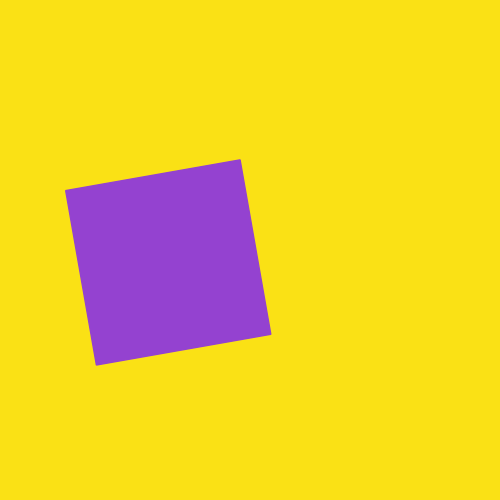
\includegraphics[width=0.35\linewidth]{imgs/Test_5/dataset_5/square_5501.png}
    
\includegraphics[width=0.35\linewidth]{imgs/Test_5/dataset_5/square_cut_5501.png}
    \caption{Quadrado e Quadrado Parcial}
    \label{fig:enter-label}
\end{figure}
\begin{figure}[H]
    \centering
    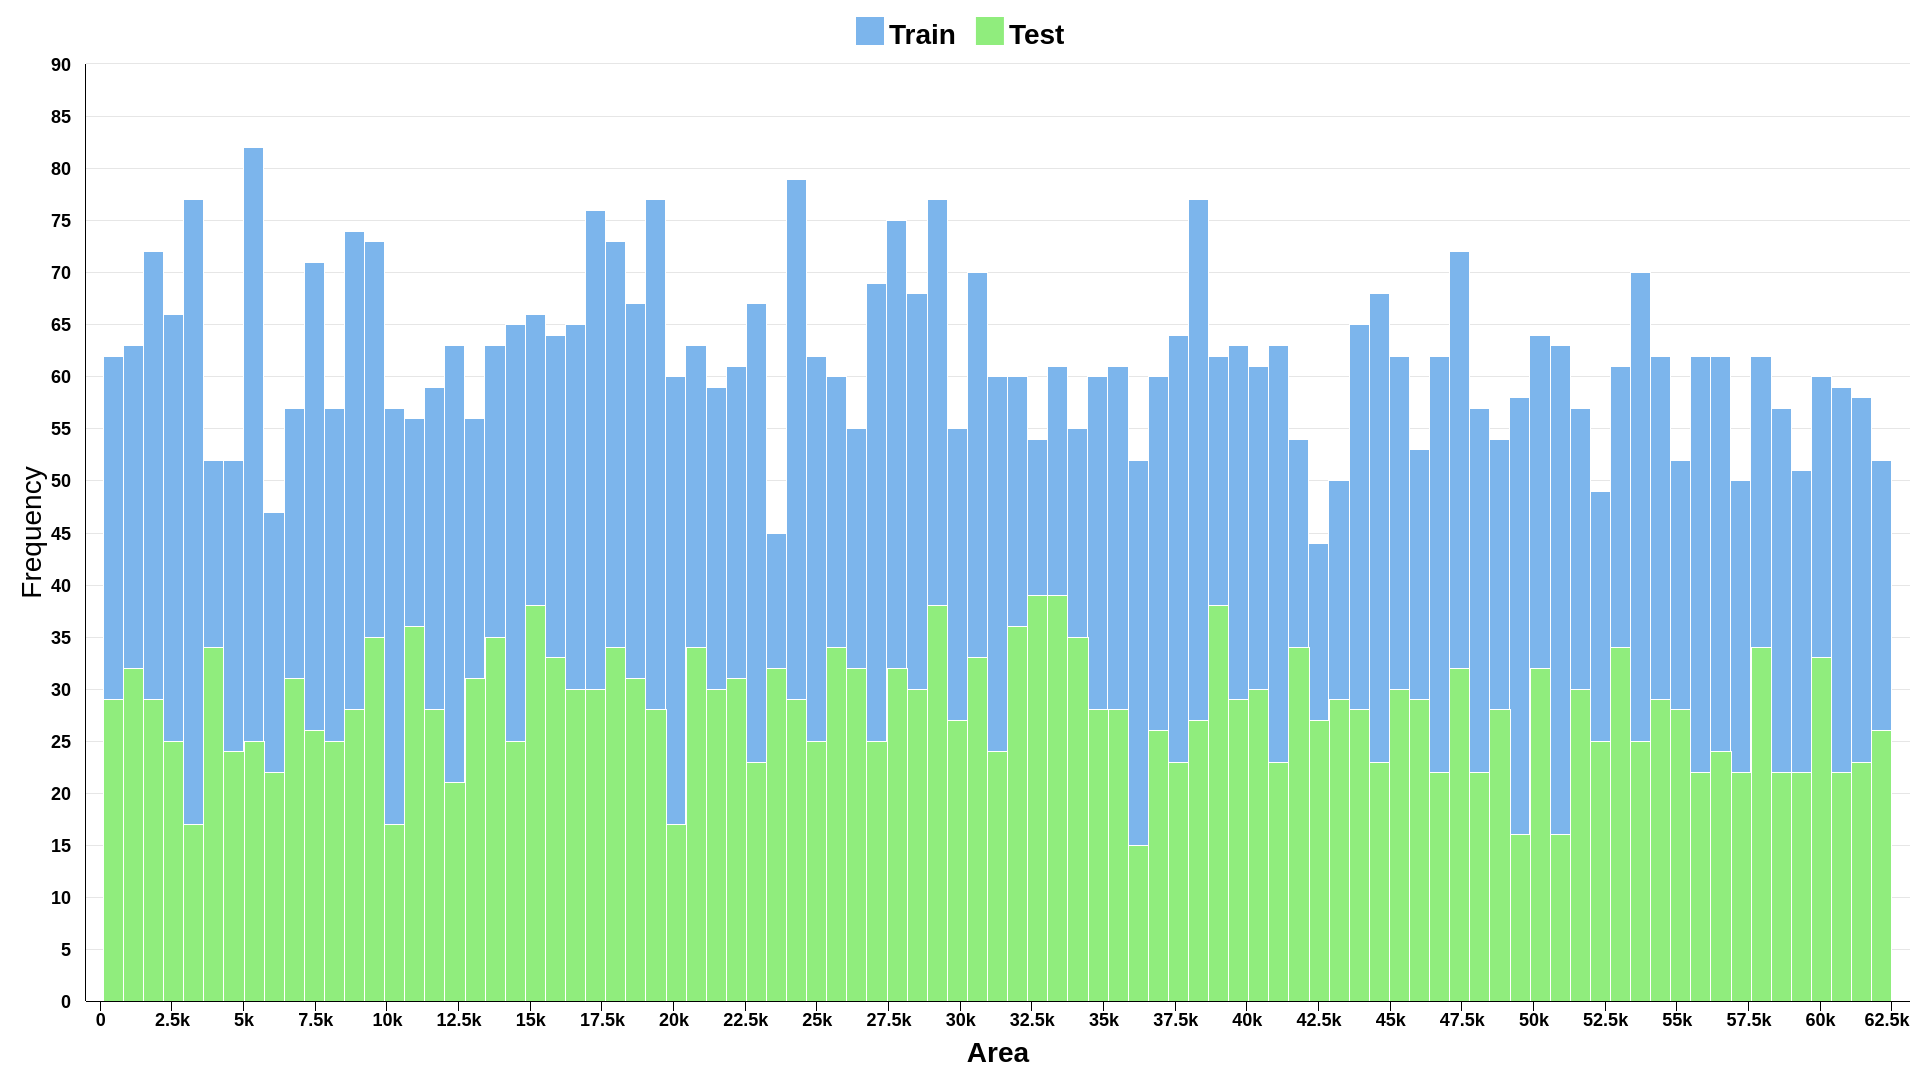
\includegraphics[width=1.0\linewidth]{imgs/Test_5/dataset_5/Squares_Area_Distribution_Hist.png}
    \caption{Distribuição da Área (Quadrados)}
    \label{fig:enter-label}
\end{figure}
\begin{figure}[H]
    \centering
    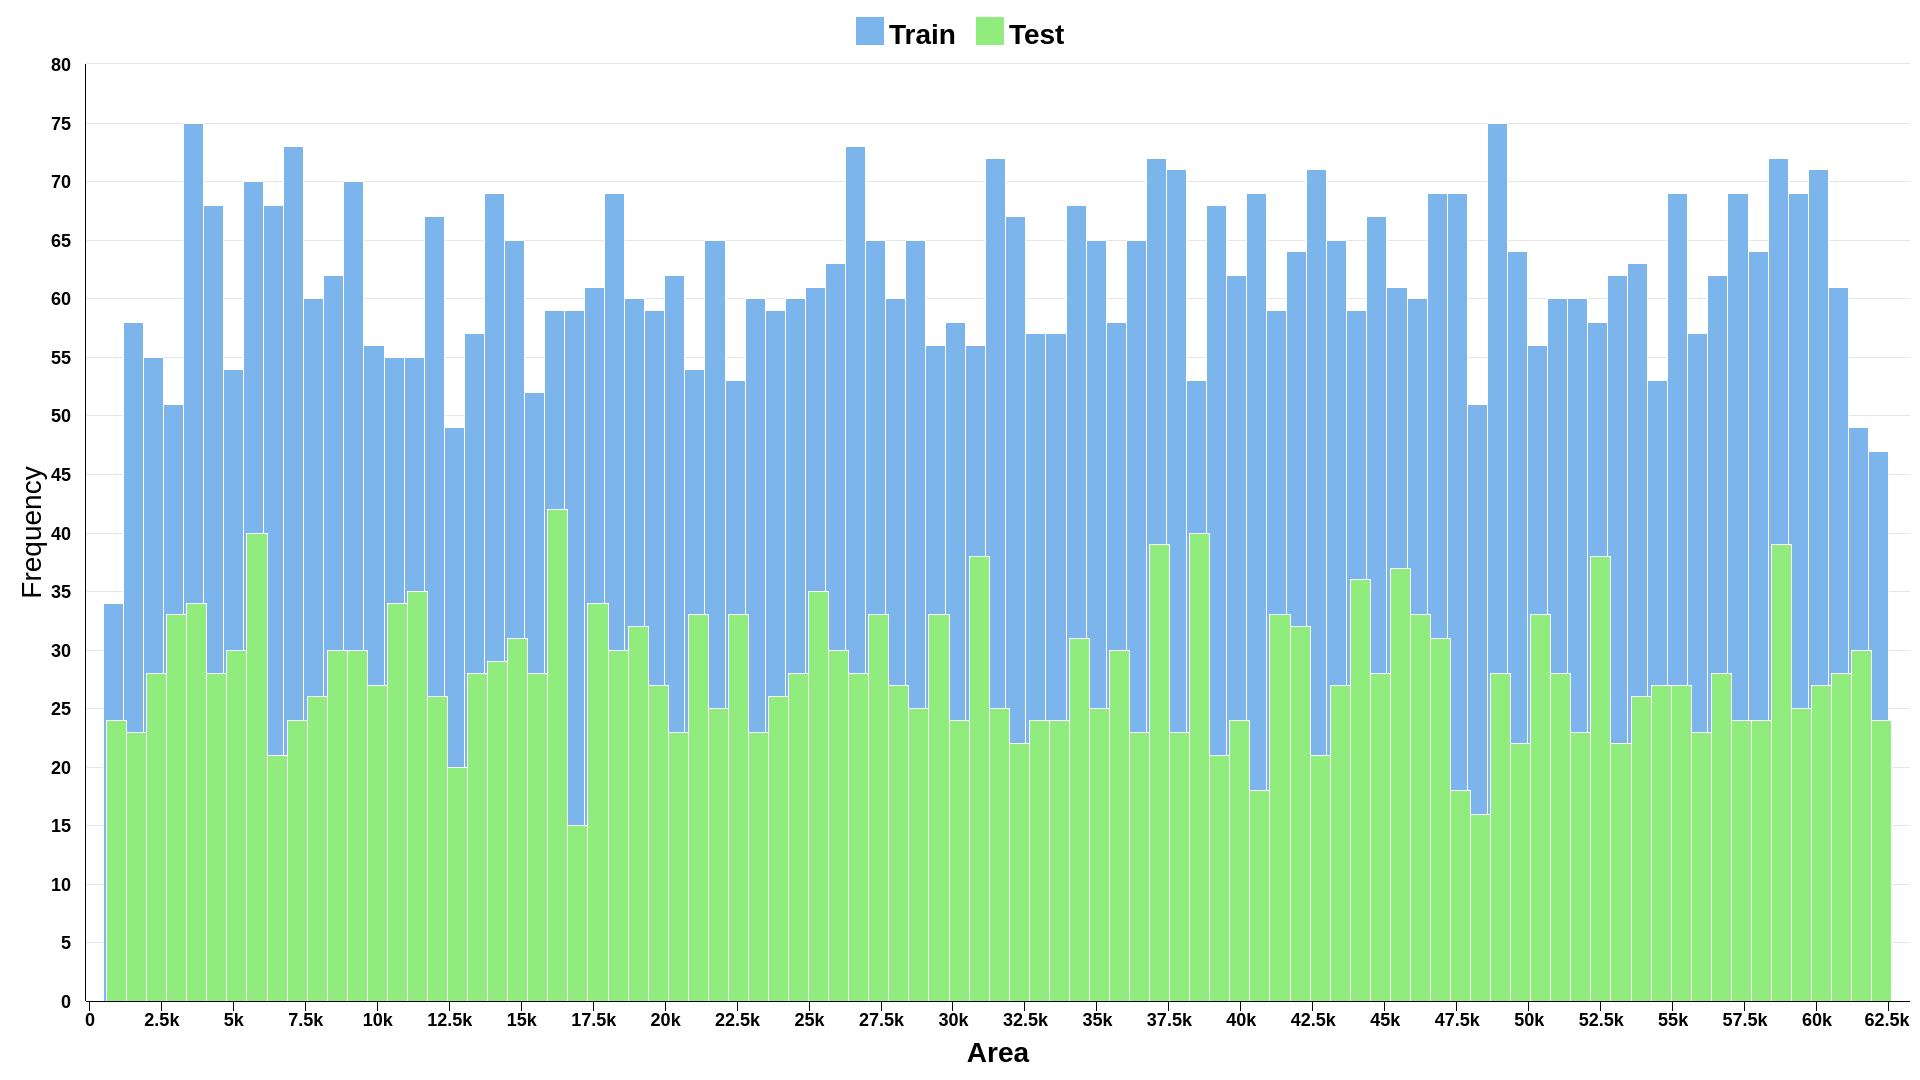
\includegraphics[width=1.0\linewidth]{imgs/Test_5/dataset_5/Partial_Squares_Area_Distribution_Hist.png}
    \caption{Distribuição da Área Visivel (Quadrados Parcial)}
    \label{fig:enter-label}
\end{figure}

\subsection{Treino}

\begin{figure}[H]
    \centering
    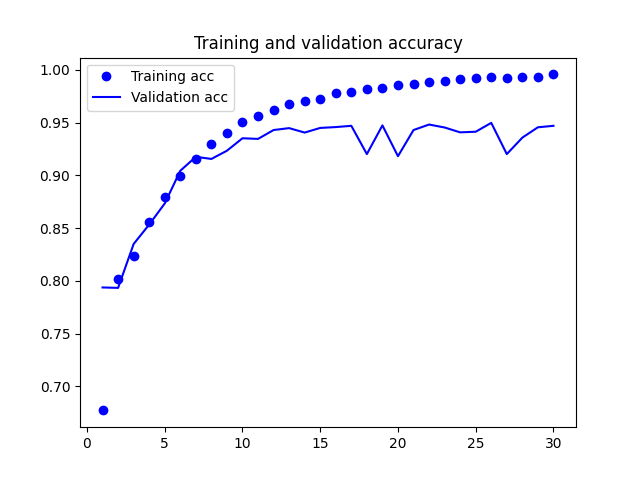
\includegraphics[width=\textwidth]{imgs/Test_5/dataset_5/train_test_acc.png}
    \caption{Acurácia de Validação e de Treino}
    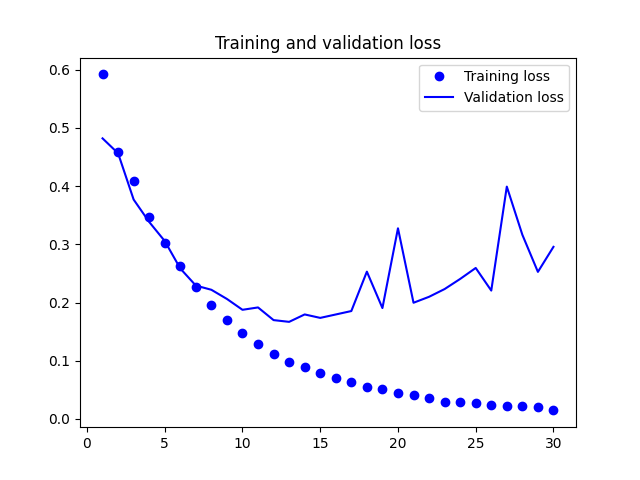
\includegraphics[width=\textwidth]{imgs/Test_5/dataset_5/train_test_loss.png}
    \caption{Perda de Validação e de Treino}
    \label{fig:sub2}
\end{figure}

Foram feitas 30 épocas, alcançando a melhor \texttt{val\_acc} na época 13 de \(94.70\%\).

\subsection{Amostras Mal Classificadas}

No total foram mal classificadas 265 (5.3\% ) imagens, sendo 95 (36\%) delas quadrados normais e as restantes 170 (64\%) quadrados parciais. 

\subsection{Matriz de Confusão}

\begin{table}[H]
\centering
\begin{tabular}{l|c c}
                   & Quadrados & Quadrados Parciais \\
\hline
Quadrados          & 2405         & 170                  \\
Quadrados Parciais & 95           & 2330                  \\
\end{tabular}
\end{table}

\subsection{Metricas de Avaliação}

\begin{table}[H]
\centering
\begin{tabular}{|c|c|c|}
\textit{Acuracy} & \textit{Precision} & \textit{Recall} \\
0.9470 & 0.9470 & 0.9470  \\
\end{tabular}
\end{table}

\subsection{Matriz de Correlação}

\subsection{Conclusão de Teste}
    Bla bla bla


\section{Teste 5.1}
\subsection{Objetivo}
\subsection{Dataset}
\subsection{Treino}
\subsection{Amostras Mal Classificadas}
\subsection{Matriz de Confusão}
\subsection{Metricas de Avaliação}
\subsection{Matriz de Correlação}
\subsection{Conclusão de Teste}
    Bla bla bla


\section{Teste 6}
\subsection{Objetivo}
\subsection{Dataset}
\subsection{Treino}
\subsection{Amostras Mal Classificadas}
\subsection{Matriz de Confusão}
\subsection{Metricas de Avaliação}
\subsection{Matriz de Correlação}
\subsection{Conclusão de Teste}
    Bla bla bla


\section{Teste 6.1}
\subsection{Objetivo}
\subsection{Dataset}
\subsection{Treino}
\subsection{Amostras Mal Classificadas}
\subsection{Matriz de Confusão}
\subsection{Metricas de Avaliação}
\subsection{Matriz de Correlação}
\subsection{Conclusão de Teste}
    Bla bla bla

section{Teste 7}
\subsection{Objetivo}
    O Teste 7 consiste em descobrir quem está mais á direita se o quadrado ou um circulo,estes têm o tamanho igual.
\subsection{Dataset}
O Dataset é composto por 11000 imagens de treino e 5000 de teste. Composto por 2 classes:
\subsection{Treino}
\subsection{Amostras Mal Classificadas}
\subsection{Matriz de Confusão}
\subsection{Metricas de Avaliação}
\subsection{Matriz de Correlação}
\subsection{Conclusão de Teste}
    Bla bla bla

\newpage

\section{Teste 7.1}
\subsection{Objetivo}
    Ver quem está a direita
    Tamanhos iguais
    Com Intesecções
\subsection{Dataset}
O Dataset é composto por 11000 imagens de treino e 5000 de teste. Composto por 2 classes:
\begin{itemize}
        \item Circulo à direita
        \item Quadrado à direita
    \end{itemize}
    Cada imagem tem 2 formas, contendo uma das seguintes combinações:
    \begin{itemize}
        \item Circulo com Circulo
        \item Quadrado com Quadrado
        \item Circulo com Quadrados
    \end{itemize}
    \begin{figure}[H]
        \centering
            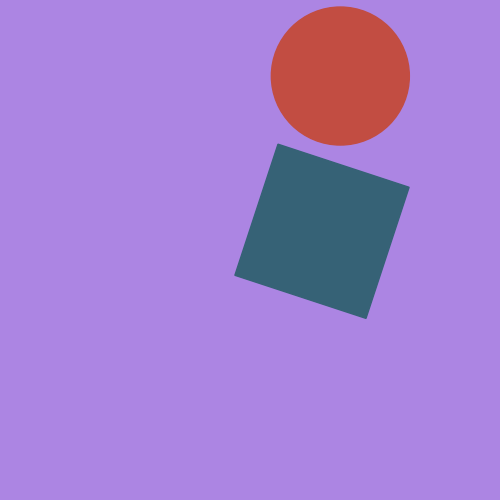
\includegraphics[width=0.25\linewidth]{imgs//Test_7/7_1/dataset/car_5629.png}
            
\includegraphics[width=0.25\linewidth]{imgs//Test_7/7_1/dataset/car_7413.png}
        \caption{Circulo à direita}
        \label{fig:enter-label}
    \end{figure}
    \begin{figure}[H]
        \centering
        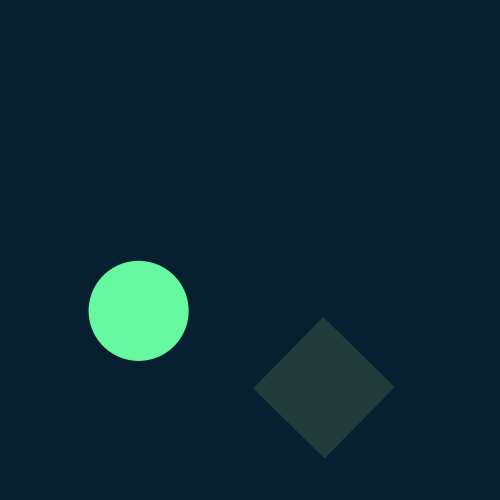
\includegraphics[width=0.25\linewidth]{imgs//Test_7/7_1/dataset/sar_5705.png}
        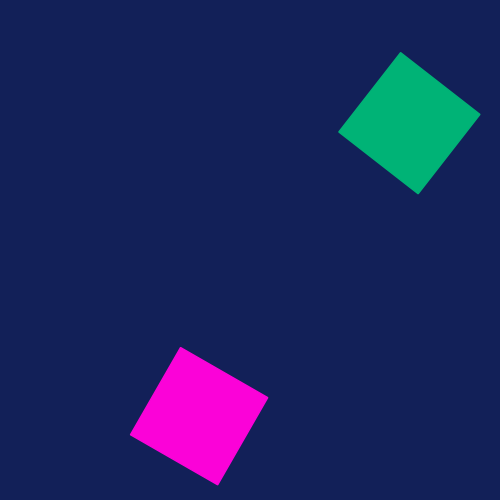
\includegraphics[width=0.25\linewidth]{imgs//Test_7/7_1/dataset/sar_7153.png}
        \caption{Quadrado à direita}
        \label{fig:enter-label}
    \end{figure}
    \begin{figure}[H]
        \centering
        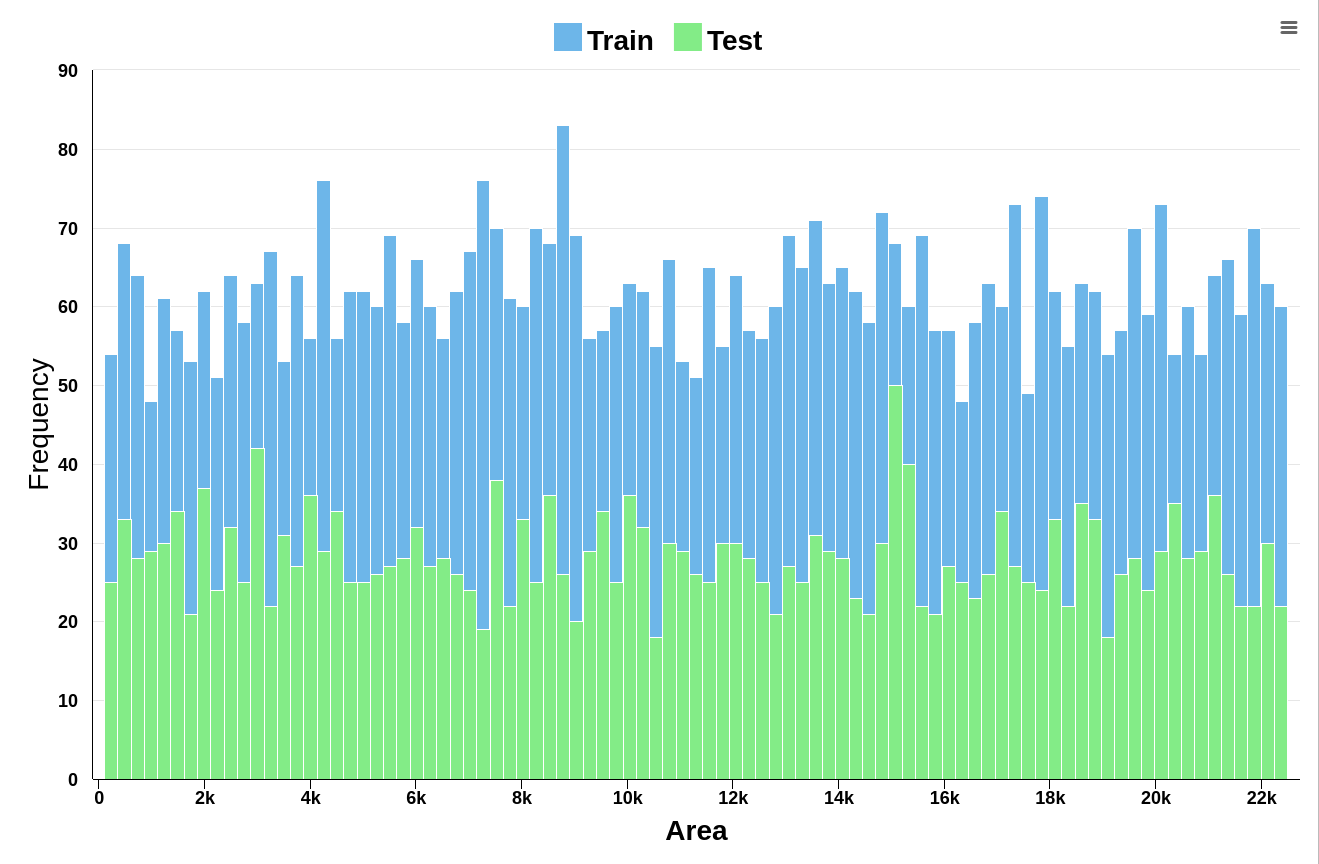
\includegraphics[width=1.0\linewidth]{imgs//Test_7/7_1/dataset/distribution_squares.png}
        \caption{Distribuição da Área (Circulos à direita)}
        \label{fig:enter-label}
    \end{figure}
    \begin{figure}[H]
        \centering
        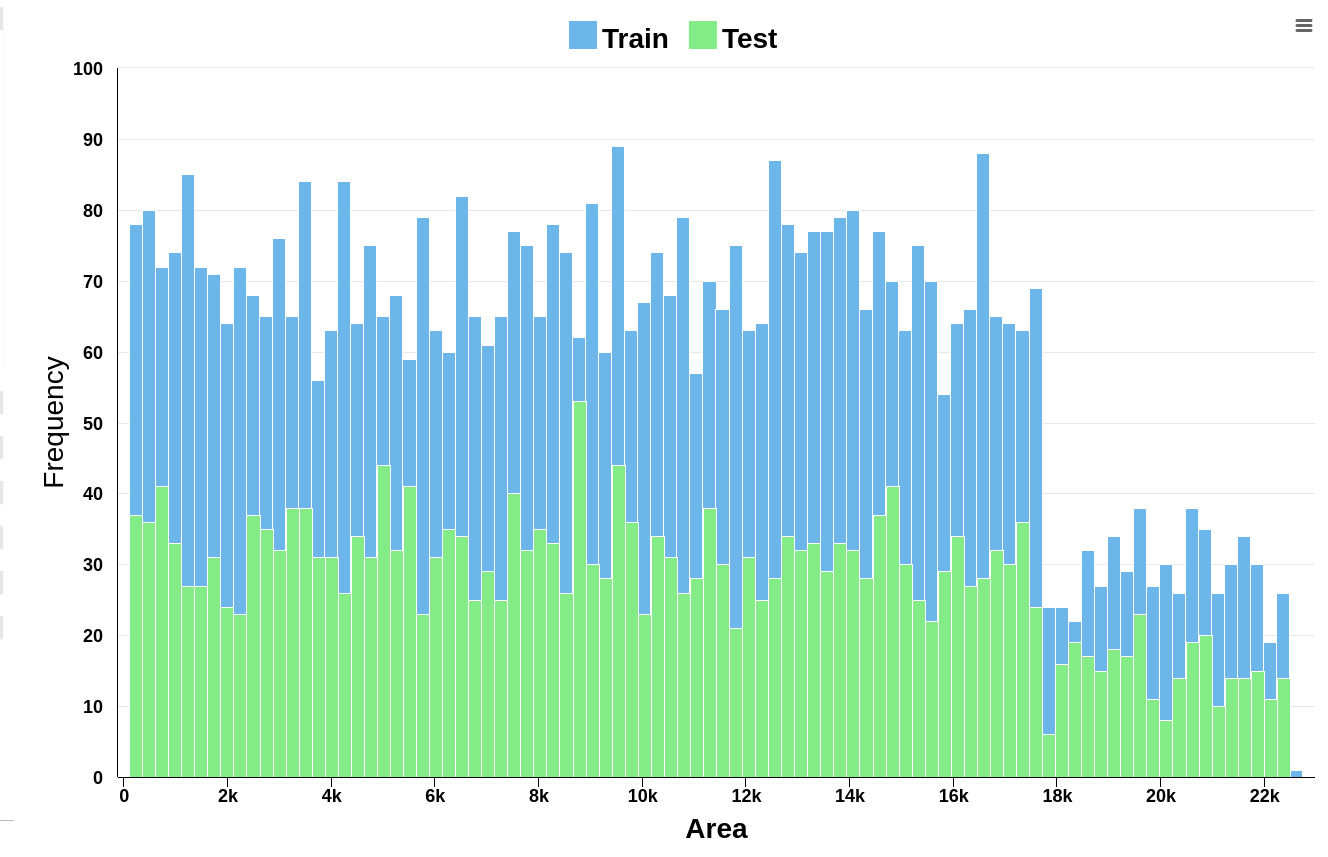
\includegraphics[width=1.0\linewidth]{imgs//Test_7/7_1/dataset/distribution_circles.png}
        \caption{Distribuição da Área (Quadrados à direita)}
        \label{fig:enter-label}
    \end{figure}
\subsection{Treino}
\begin{figure}[H]
    \centering
    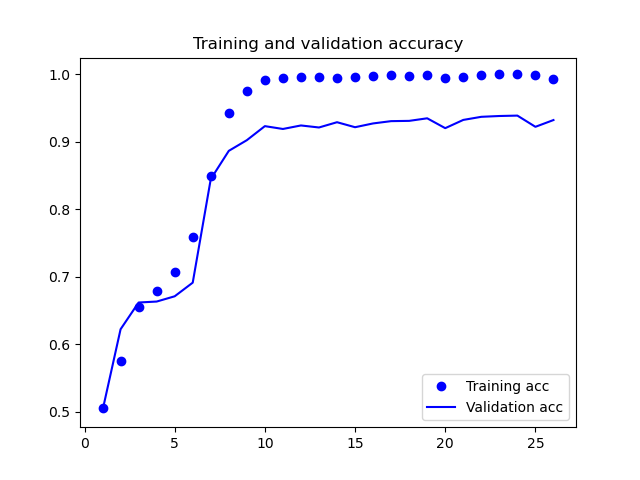
\includegraphics[width=\textwidth]{imgs//Test_7/7_1/train_test_acc.png}
    \caption{Acurácia de Validação e de Treino}
    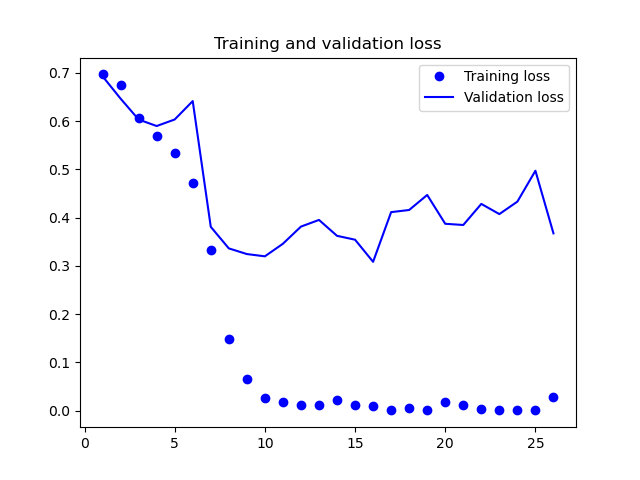
\includegraphics[width=\textwidth]{imgs//Test_7/7_1/train_test_loss.png}
    \caption{Perda de Validação e de Treino}
    \label{fig:sub2}
    Com as 26 épocas realizadas, conseguimos uma val acc de 0.9024, sendo que a melhor loss foi atingida na época 10.
\end{figure}
\subsection{Amostras Mal Classificadas}
No total foram mal classificadas 339 (13.74\% ) imagens de teste sendo:
    - 65 imagens com circulo à direita com um quadrado à esquerda
    - 44 imagens com circulo à direita e à esquerda
    - 86 imagens com quadrado à direita e com um circulo à esquerda 
    - 144 imagens com quadrado à direita e à esquerda
    

\subsection{Matriz de Confusão}

\begin{table}[H]
\centering
\begin{tabular}{l|c c}
                & Circulo à Direita & Quadrado à Direita \\ 
\hline
Circulo à Direita         & 2391         & 109                  \\
Quadrado à Direita        & 230         & 2270                 \\

\end{tabular}
\end{table}

\subsection{Metricas de Avaliação}
\subsection{Matriz de Correlação}
\subsection{Conclusão de Teste}
    Bla bla bla

\newpage

\section{Teste 7.2}
\subsection{Objetivo}
    Este teste é bastante semelhante ao teste 7, ao seja o objetivo é identificar entre um quadrado ou circulo, qual o que está mais á direita na imagem. Neste caso os tamanhos das formas podem ser diferente um do outro
\subsection{Dataset}
O Dataset é composto por 11000 imagens de treino e 5000 de teste. Composto por 2 classes:
    \begin{itemize}
        \item Circulo à direita
        \item Quadrado à direita
    \end{itemize}
    Cada imagem tem 2 formas, contendo uma das seguintes combinações:
    \begin{itemize}
        \item Circulo com Circulo
        \item Quadrado com Quadrado
        \item Circulo com Quadrados
    \end{itemize}
    \begin{figure}[H]
        \centering
            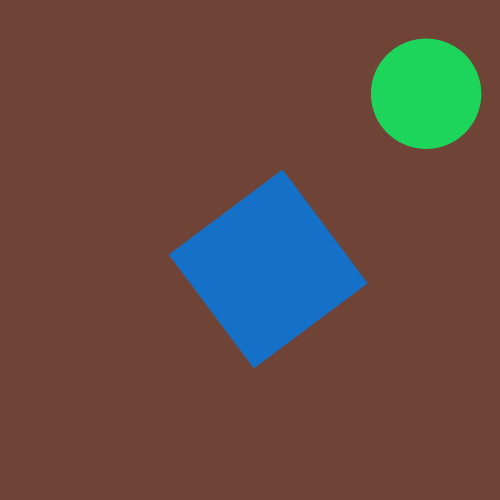
\includegraphics[width=0.25\linewidth]{imgs/Test_7/7_2/dataset/car_1.png}
            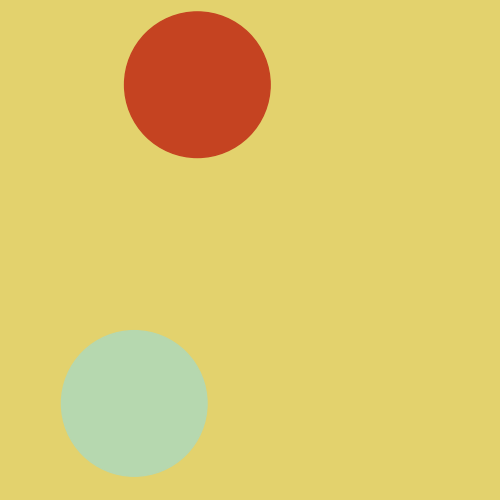
\includegraphics[width=0.25\linewidth]{imgs/Test_7/7_2/dataset/car_3116.png}
        \caption{Circulo à direita}
        \label{fig:enter-label}
    \end{figure}
    \begin{figure}[H]
        \centering
        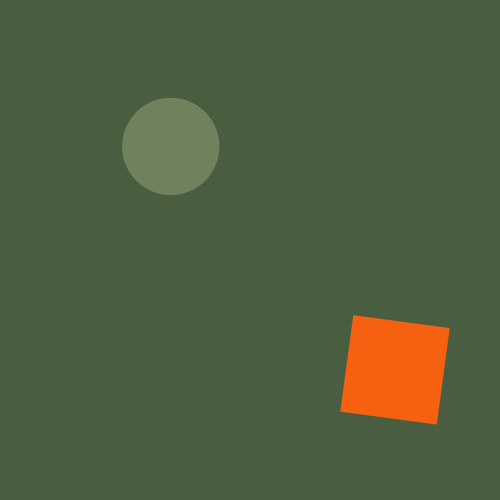
\includegraphics[width=0.25\linewidth]{imgs/Test_7/7_2/dataset/sar_9.png}
        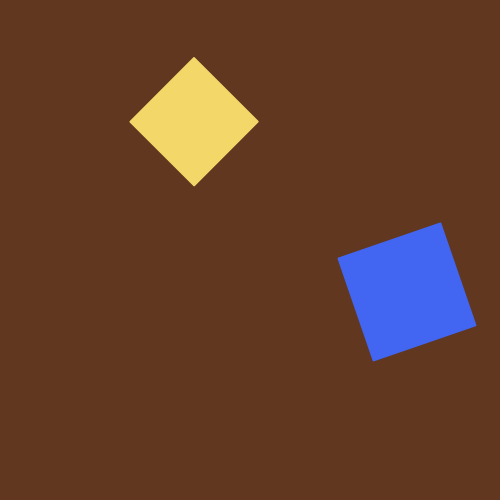
\includegraphics[width=0.25\linewidth]{imgs/Test_7/7_2/dataset/sar_3873.png}
        \caption{Quadrado à direita}
        \label{fig:enter-label}
    \end{figure}
    \begin{figure}[H]
        \centering
        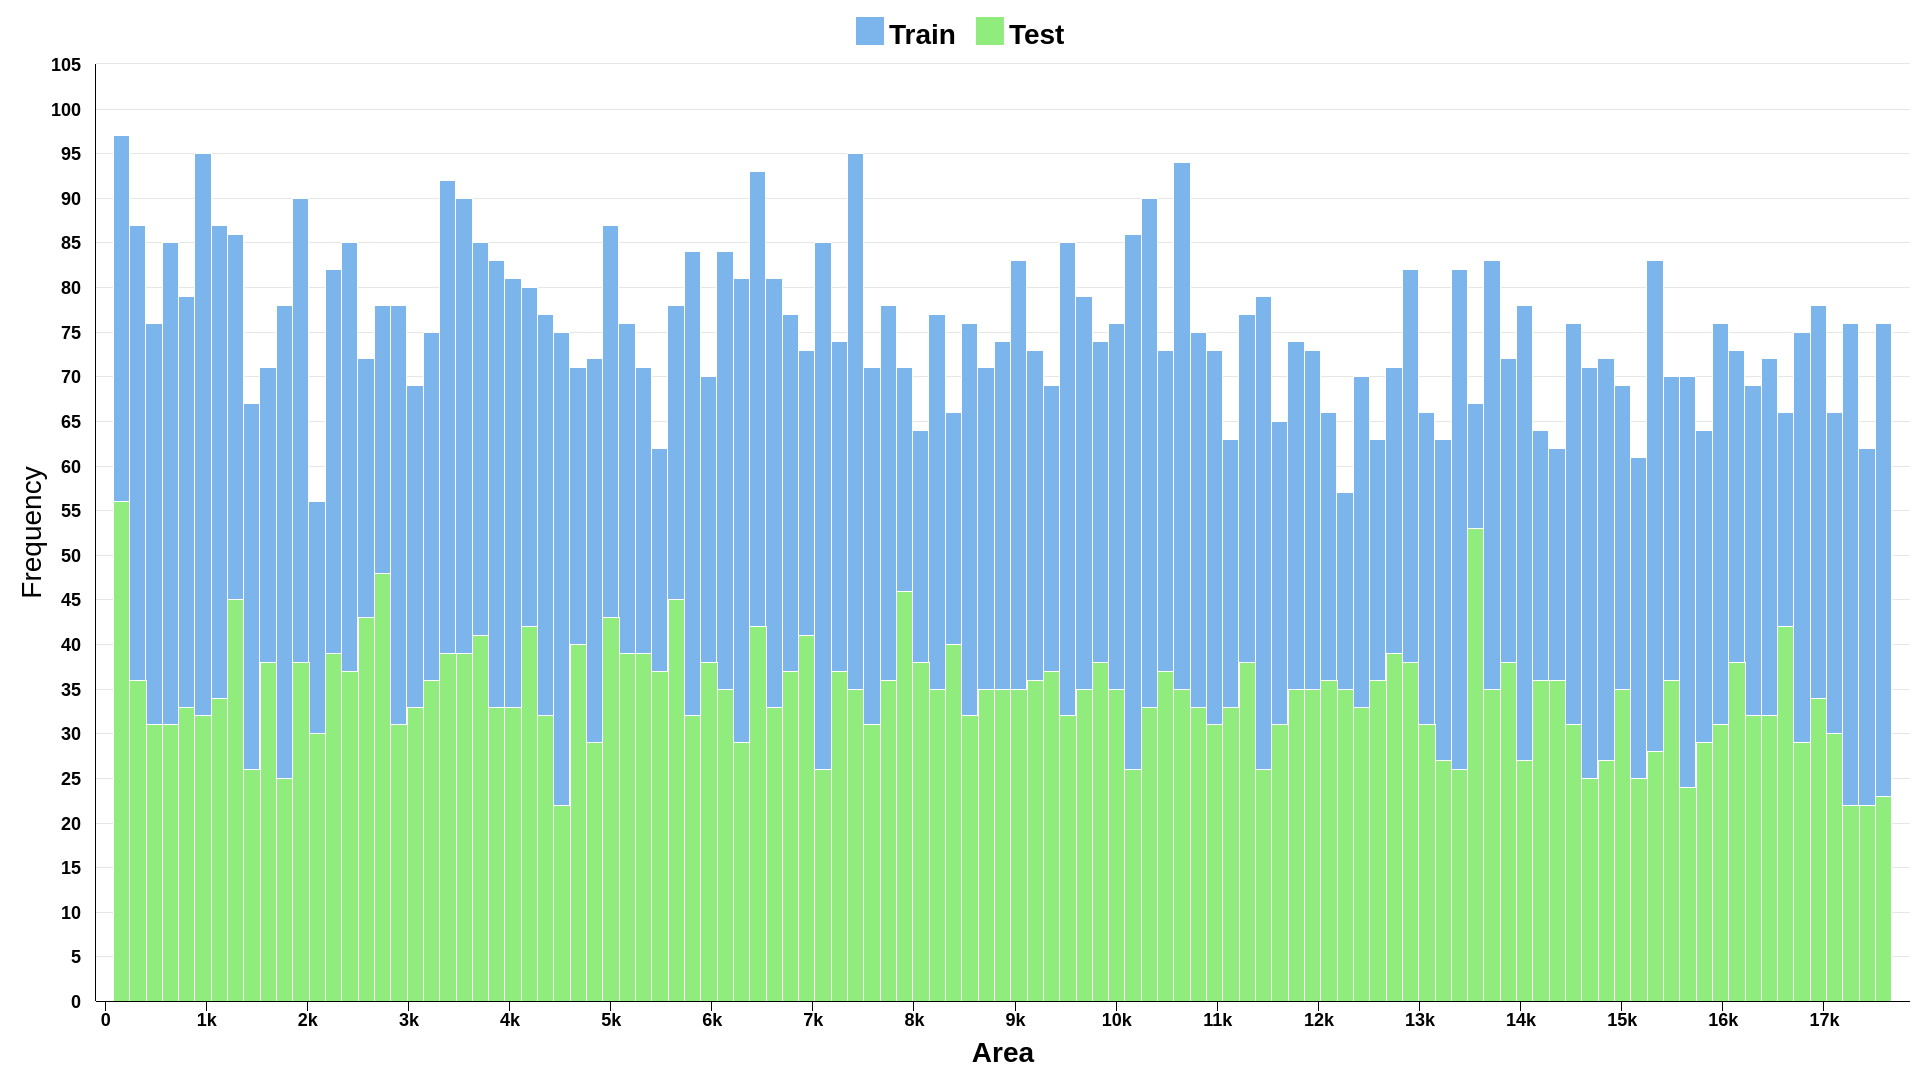
\includegraphics[width=1.0\linewidth]{imgs/Test_7/7_2/dataset/car_ci_distribution_hist.png}
        \caption{Distribuição da Área (Circulos à direita)}
        \label{fig:enter-label}
    \end{figure}
    \begin{figure}[H]
        \centering
        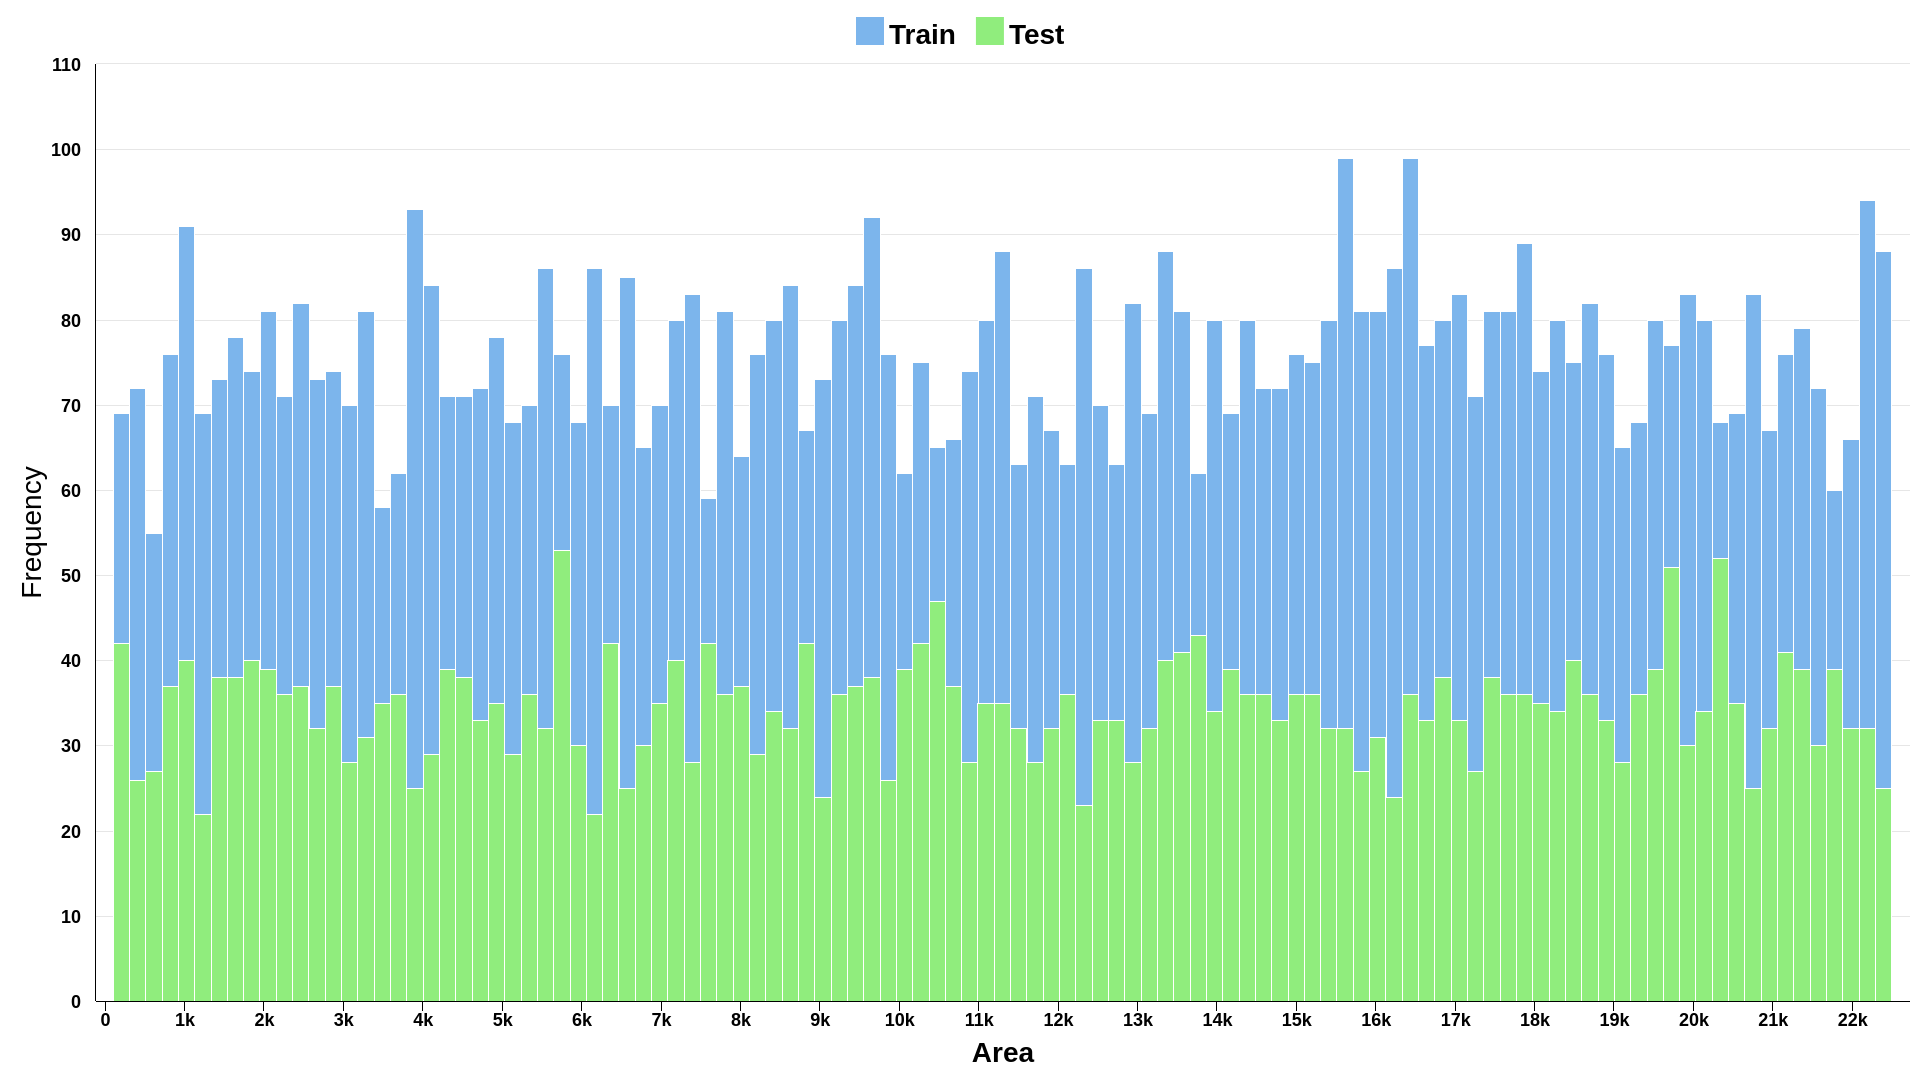
\includegraphics[width=1.0\linewidth]{imgs/Test_7/7_2/dataset/sar_sq_distribution_hist.png}
        \caption{Distribuição da Área (Quadrados à direita)}
        \label{fig:enter-label}
    \end{figure}
\subsection{Treino}
\begin{figure}[H]
    \centering
    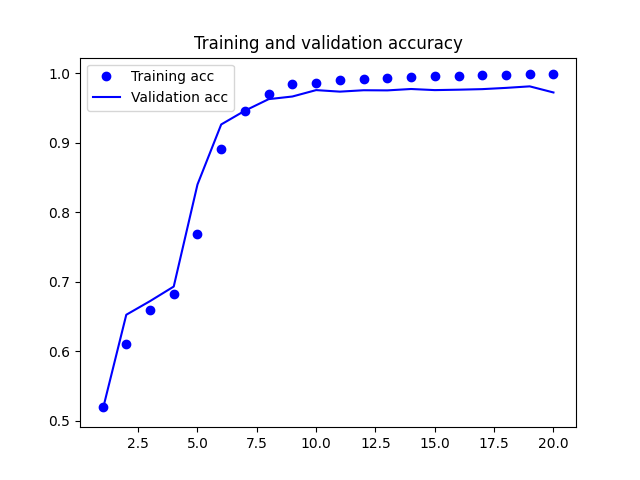
\includegraphics[width=\textwidth]{imgs/Test_7/7_2/train_test_acc.png}
    \caption{Acurácia de Validação e de Treino}
    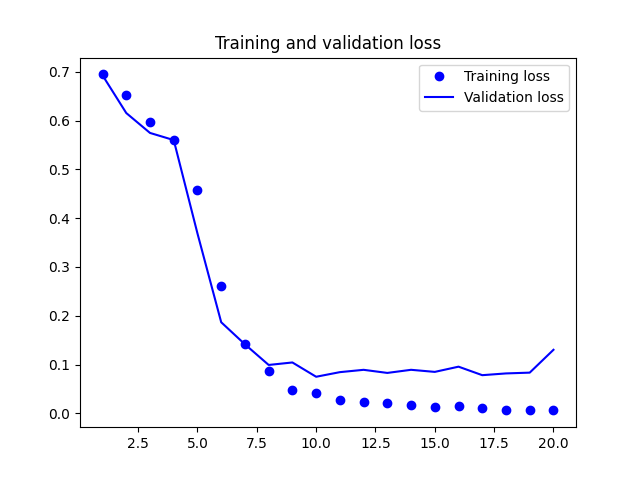
\includegraphics[width=\textwidth]{imgs/Test_7/7_2/train_test_loss.png}
    \caption{Perda de Validação e de Treino}
    \label{fig:sub2}
    Com as 20 épocas realizadas, conseguimos uma val acc de 0.9720, sendo que a melhor loss foi atingida na época 10.
\end{figure}

\subsection{Amostras Mal Classificadas}

No total foram mal classificadas 140 (2.8\% ) imagens sendo:
 \begin{itemize}
    \item 0 imagens com circulo à direita com um quadrado à esquerda
    \item 13 imagens com circulo à direita e à esquerda
    \item 45 imagens com quadrado à direita e com um circulo à esquerda 
    \item 52 imagens com quadrado à direita e à esquerda
\end{itemize}
    

\subsection{Matriz de Confusão}

\begin{table}[H]
\centering
\begin{tabular}{l|c c}
                & Circulo à Direita & Quadrado à Direita \\
\hline
Circulo à Direita         & 2406         & 97                  \\
Quadrado à Direita        & 43         & 2457                 \\

\end{tabular}
\end{table}

\subsection{Análise}
\begin{figure}[H]
    \centering
    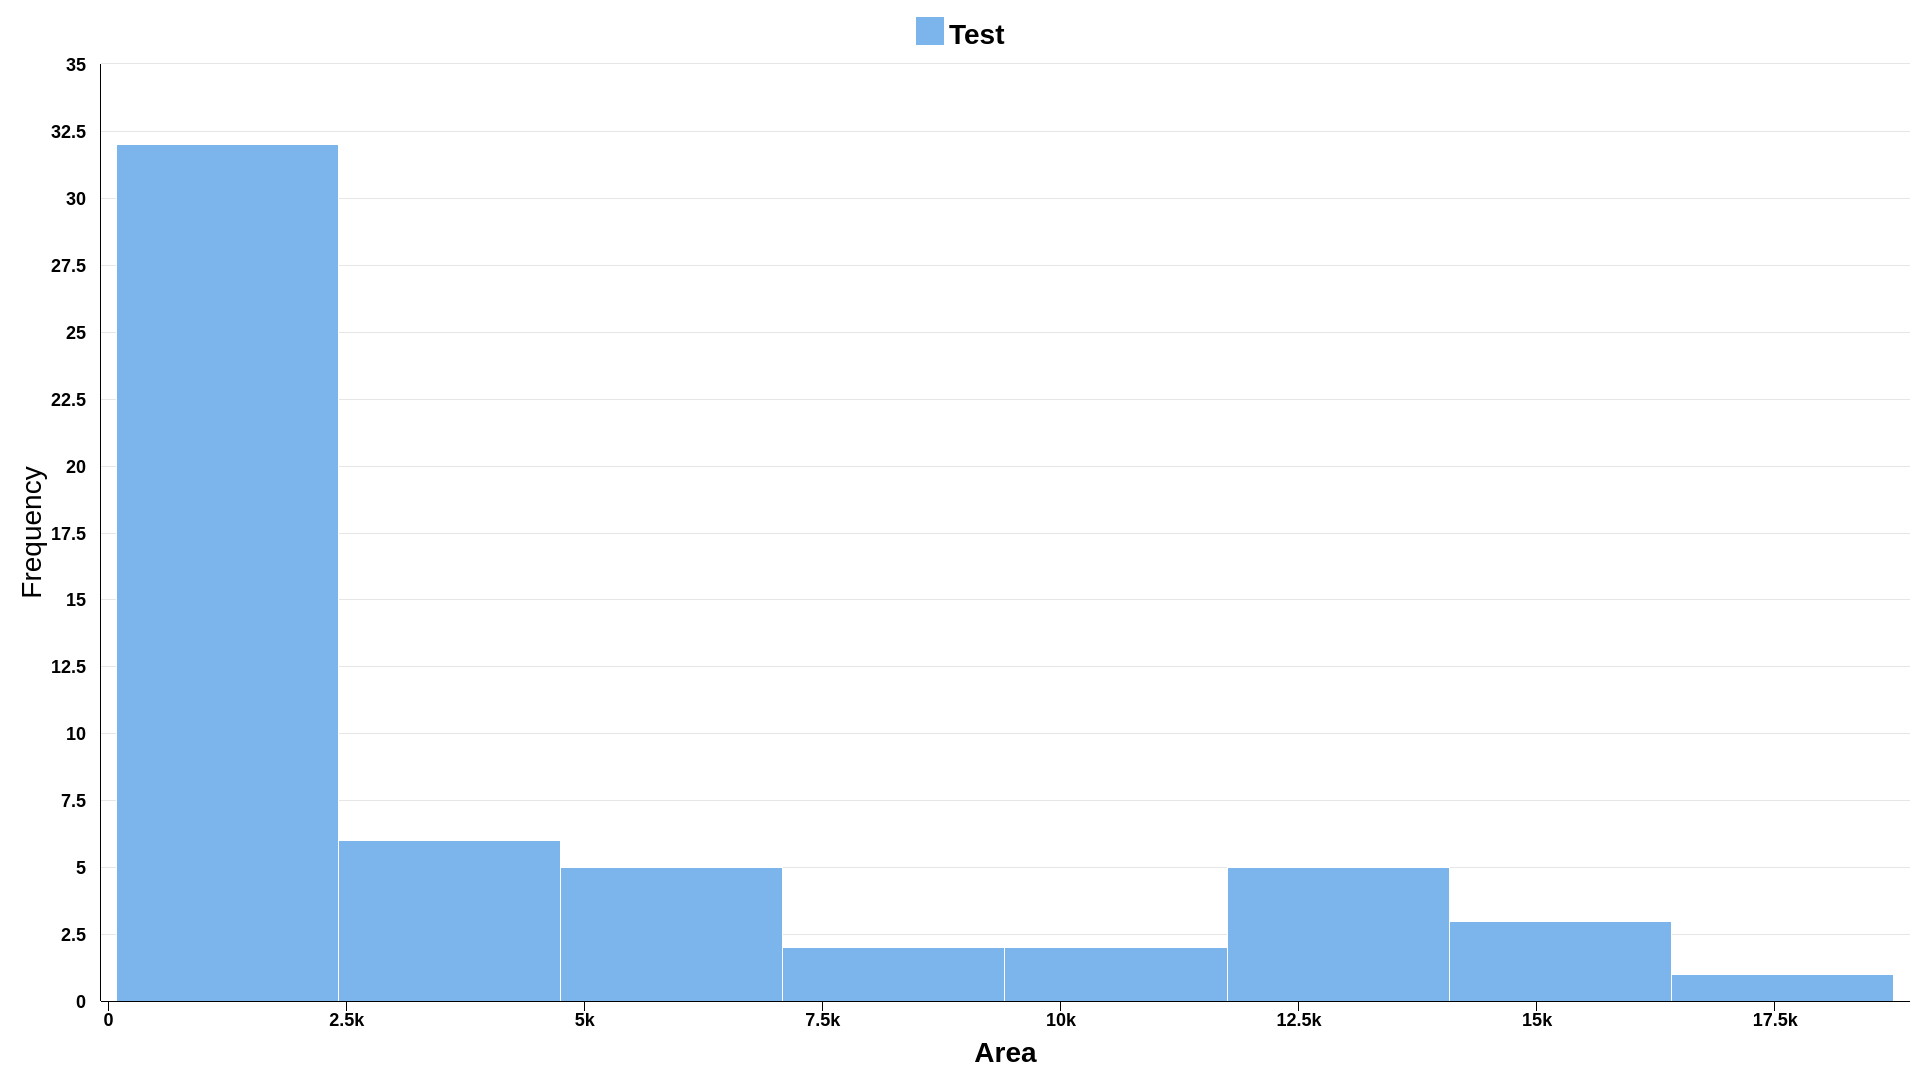
\includegraphics[width=\textwidth]{imgs/Test_7/7_2/failed/car_ci_failed_area_hist.png}
    \caption{Distribuição da Área dos Circulos à direita }
    \label{fig:sub2}
\end{figure}

\begin{figure}[H]
    \centering
    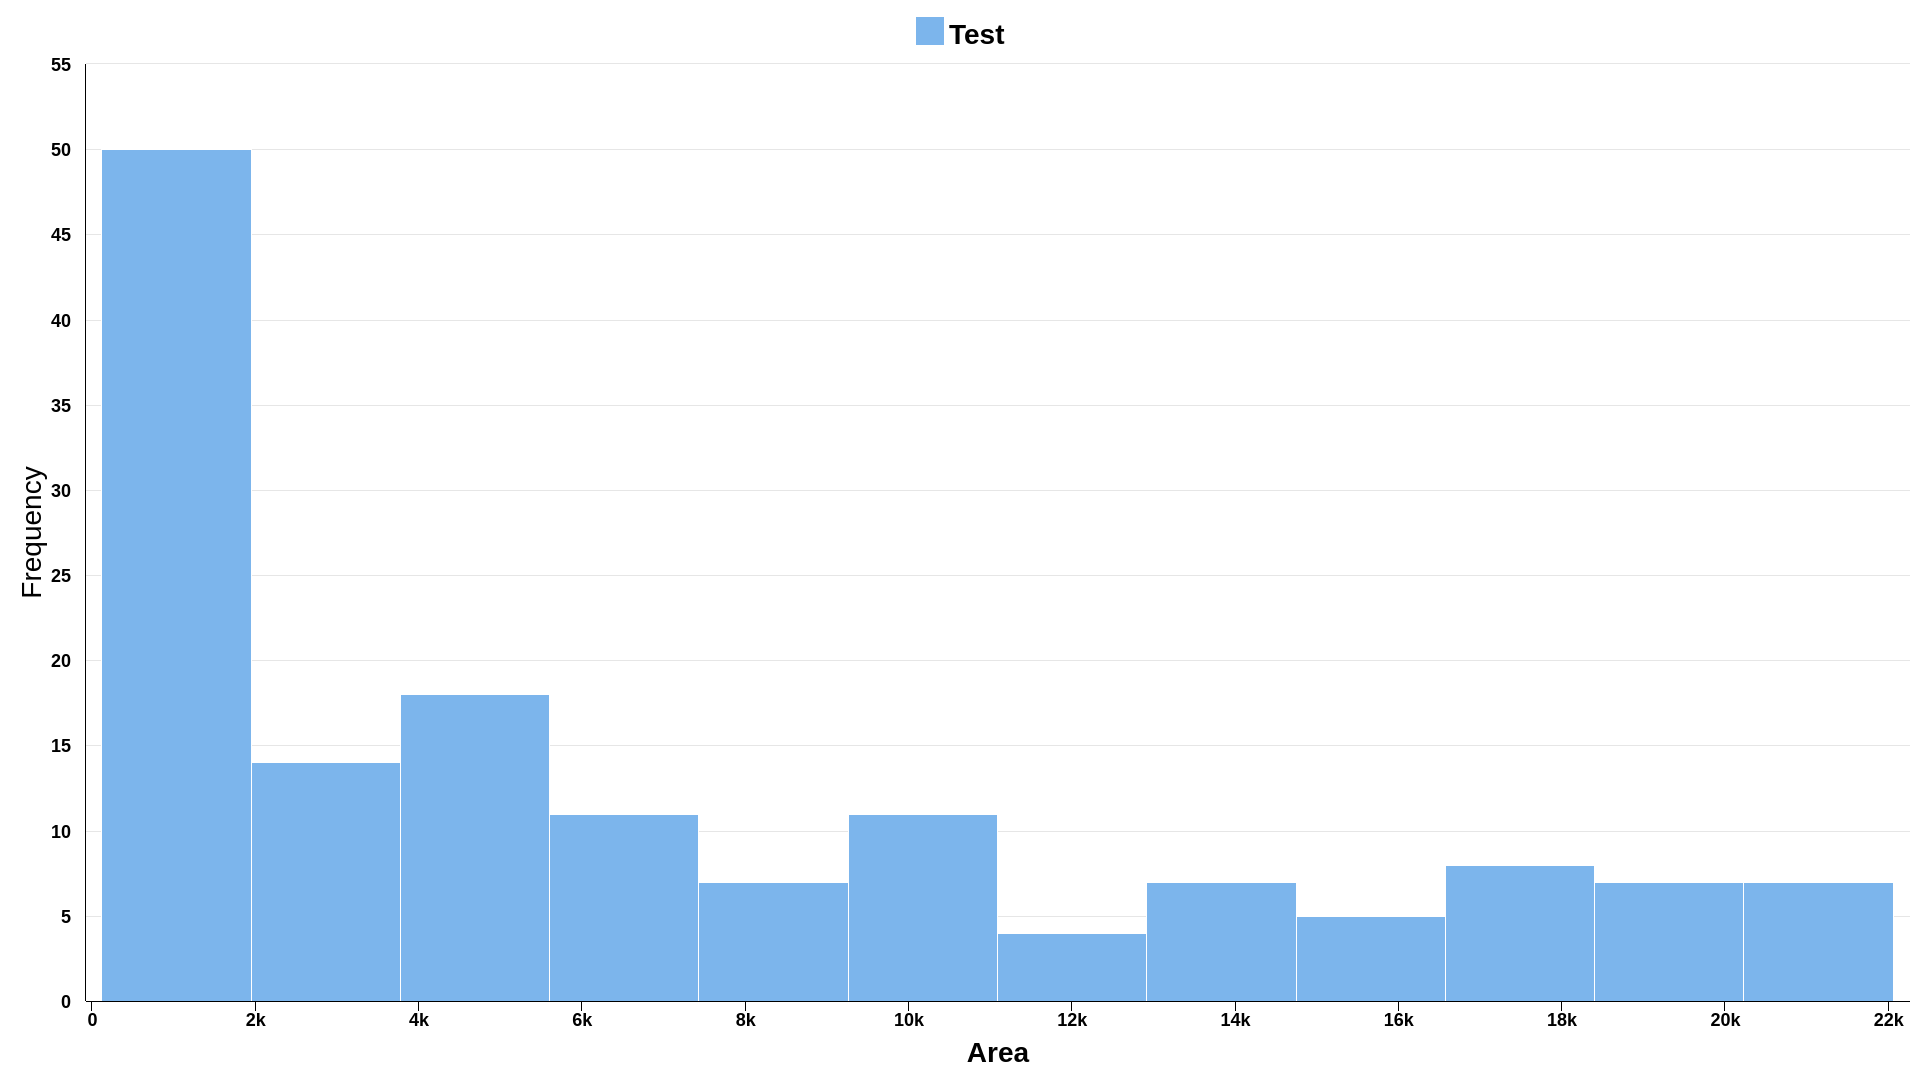
\includegraphics[width=\textwidth]{imgs/Test_7/7_2/failed/sar_sq_failed_area_hist.png}
    \caption{Distribuição da Área dos Quadrados à direita }
    \label{fig:sub2}
\end{figure}

\begin{figure}[H]
    \centering
    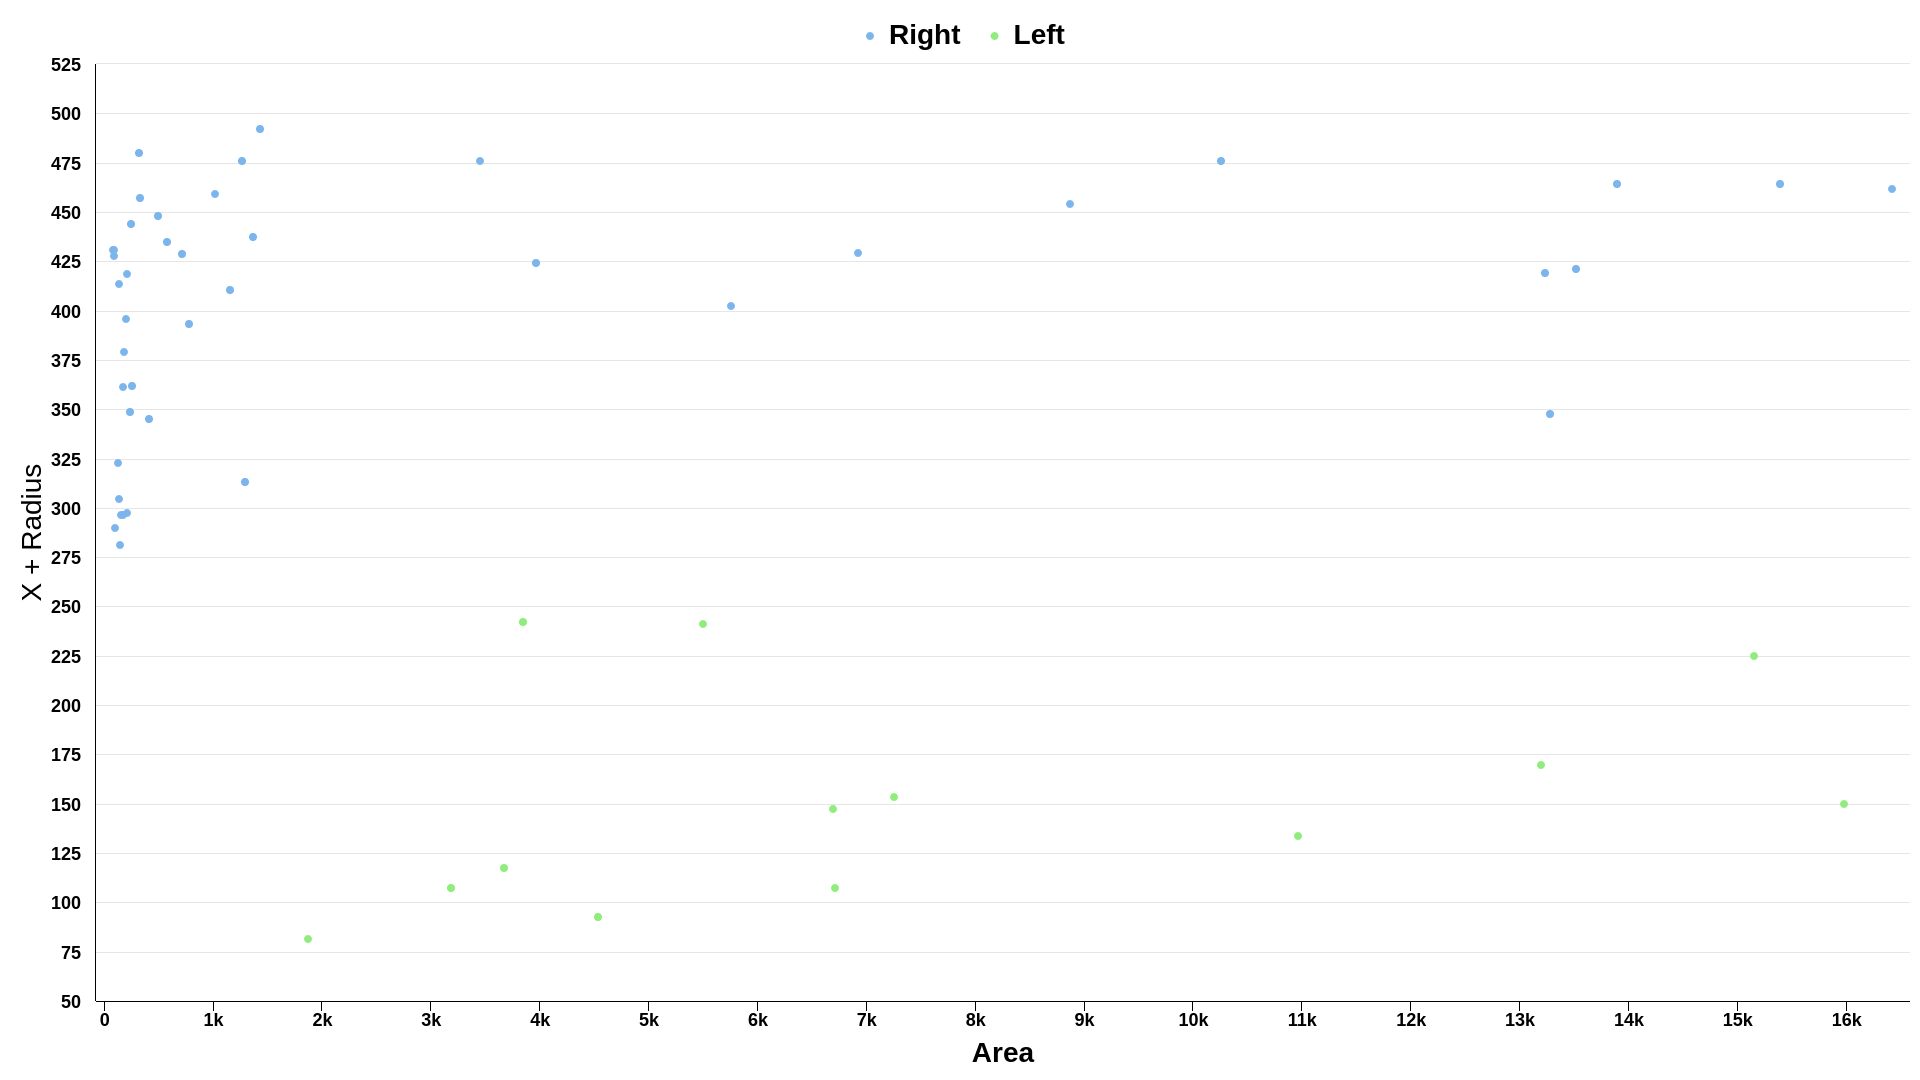
\includegraphics[width=\textwidth]{imgs/Test_7/7_2/failed/car_ci_failed_right_left_scatter.png}
    \caption{Scatter dos circulos, em imagens de circulos à direita}
    \label{fig:sub2}
\end{figure}

\begin{figure}[H]
    \centering
    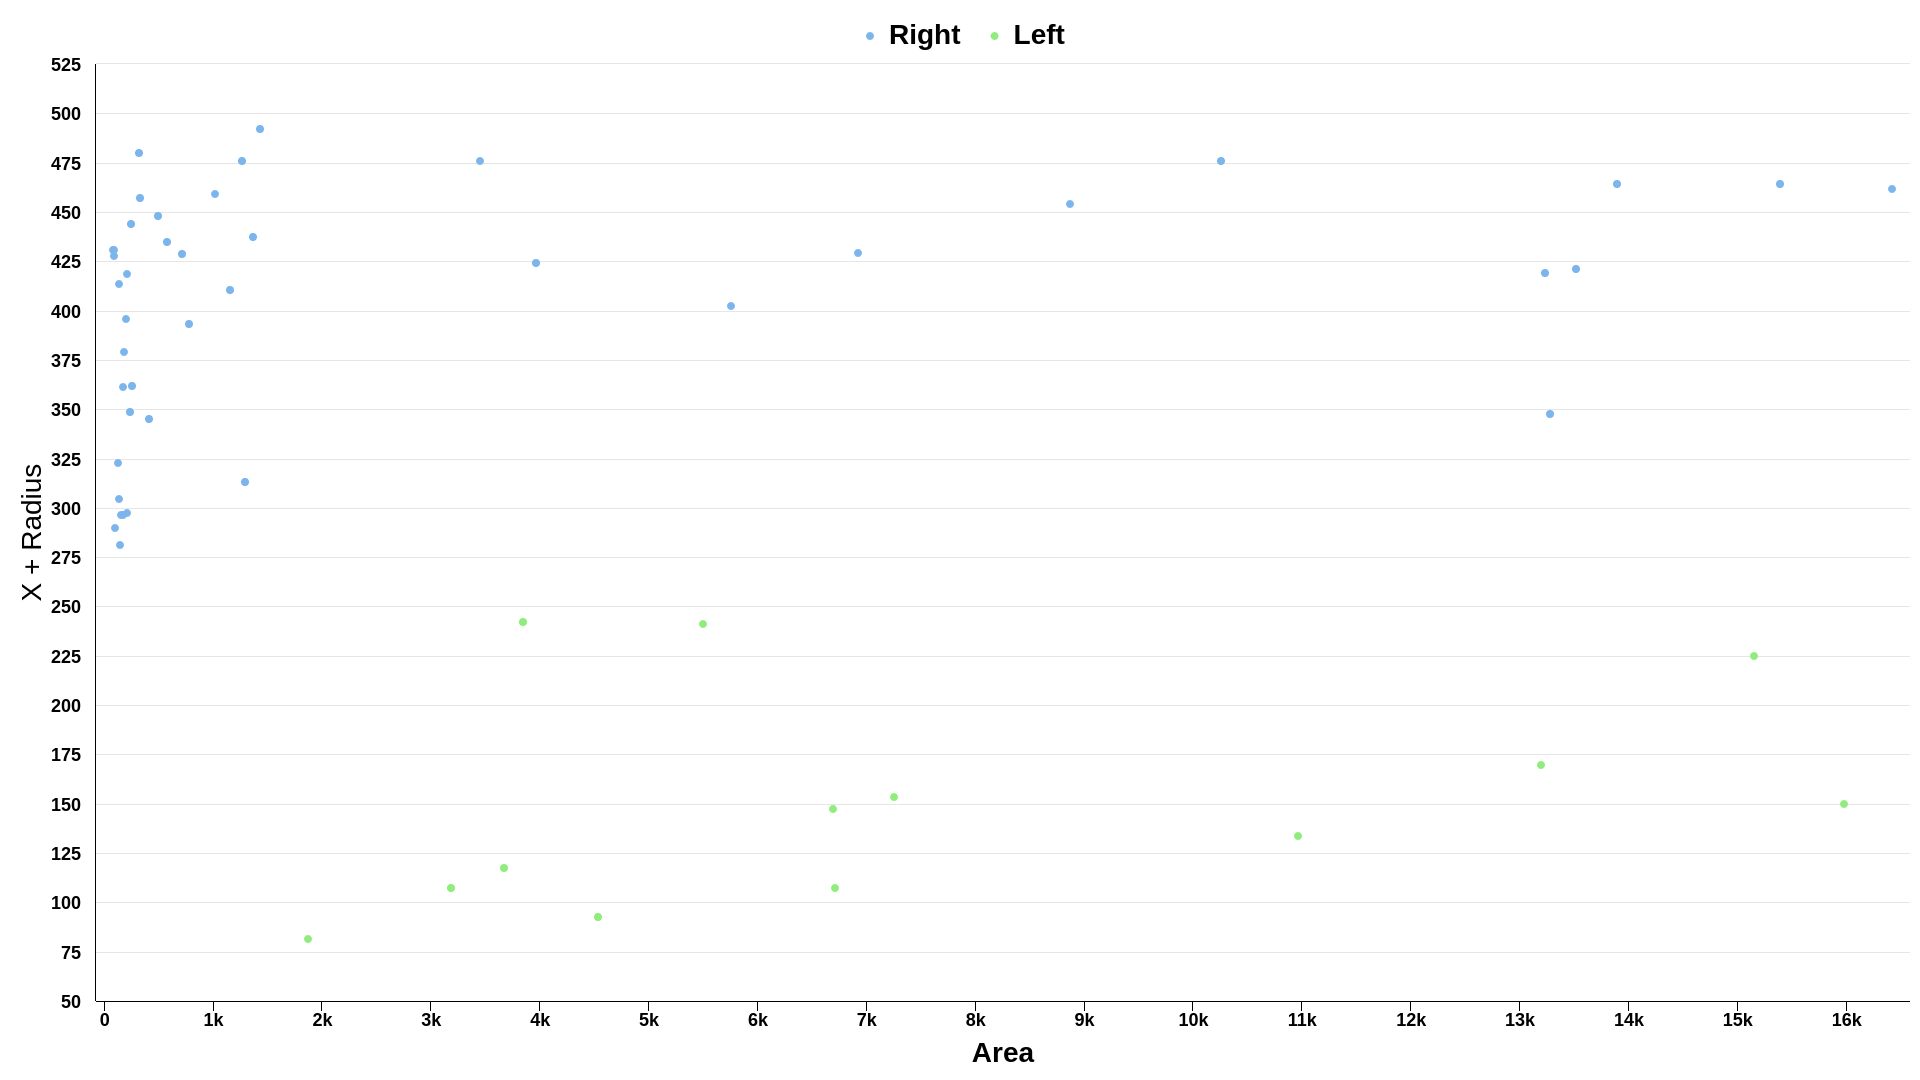
\includegraphics[width=\textwidth]{imgs/Test_7/7_2/failed/car_ci_failed_right_left_scatter.png}
    \caption{Scatter dos quadrados, em imagens de quadrados à direita}
    \label{fig:sub2}
\end{figure}

Como podemos ver partir dos histogramas, o que causa o modelo ao engano é quando numa imagem está presente circulos ou quadrados muito pequenos. Um pormenor que é possivel observar, principalmente no scatter dos quadrados, é que o que está á esquerda não influencia muito devido ao tamanho, o tamanho só influencia caso esse esteja à direita


\section{Teste 7.3}
\subsection{Objetivo}
    Ver quem está a direita
    Tamanhos diferentes
    Com Intersecções


\section{Teste 8-ALT}
\subsection{Objetivo}
       Circlos com Circlos
       Ver Porpoção
    
    

\section{Teste 8}
\subsection{Objetivo}

\subsection{Dataset}
    O Dataset é composto por 5500 imagens de treino e 2500 de teste. Composto por apenas imagens com 1 circulo.
    Este dataset foi tambem utilizado no teste 5_1.
    
   
        \begin{figure}[H]
        \centering
        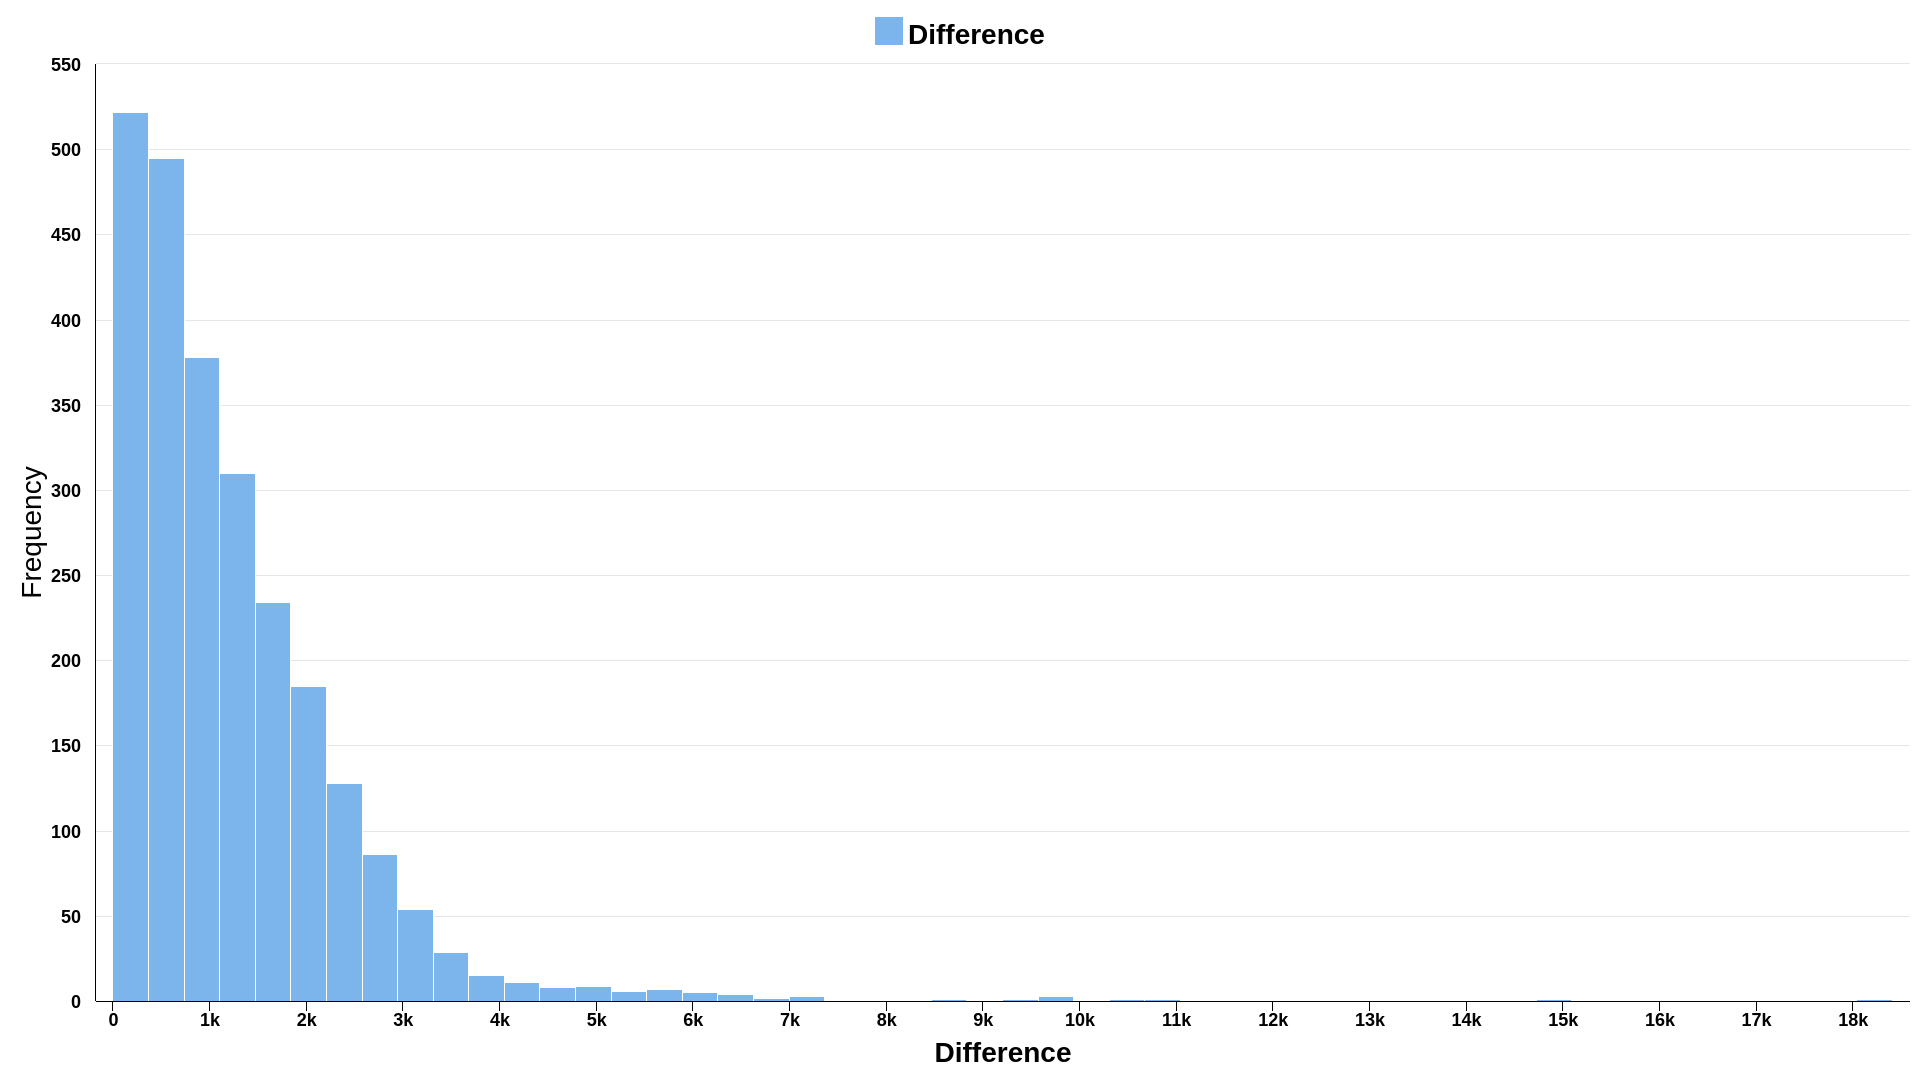
\includegraphics[width=1.0\linewidth]{imgs/Test_8/area_diference_hist.png}

        \label{fig:enter-label}
    \end{figure}
    
       
        \begin{figure}[H]
        \centering
        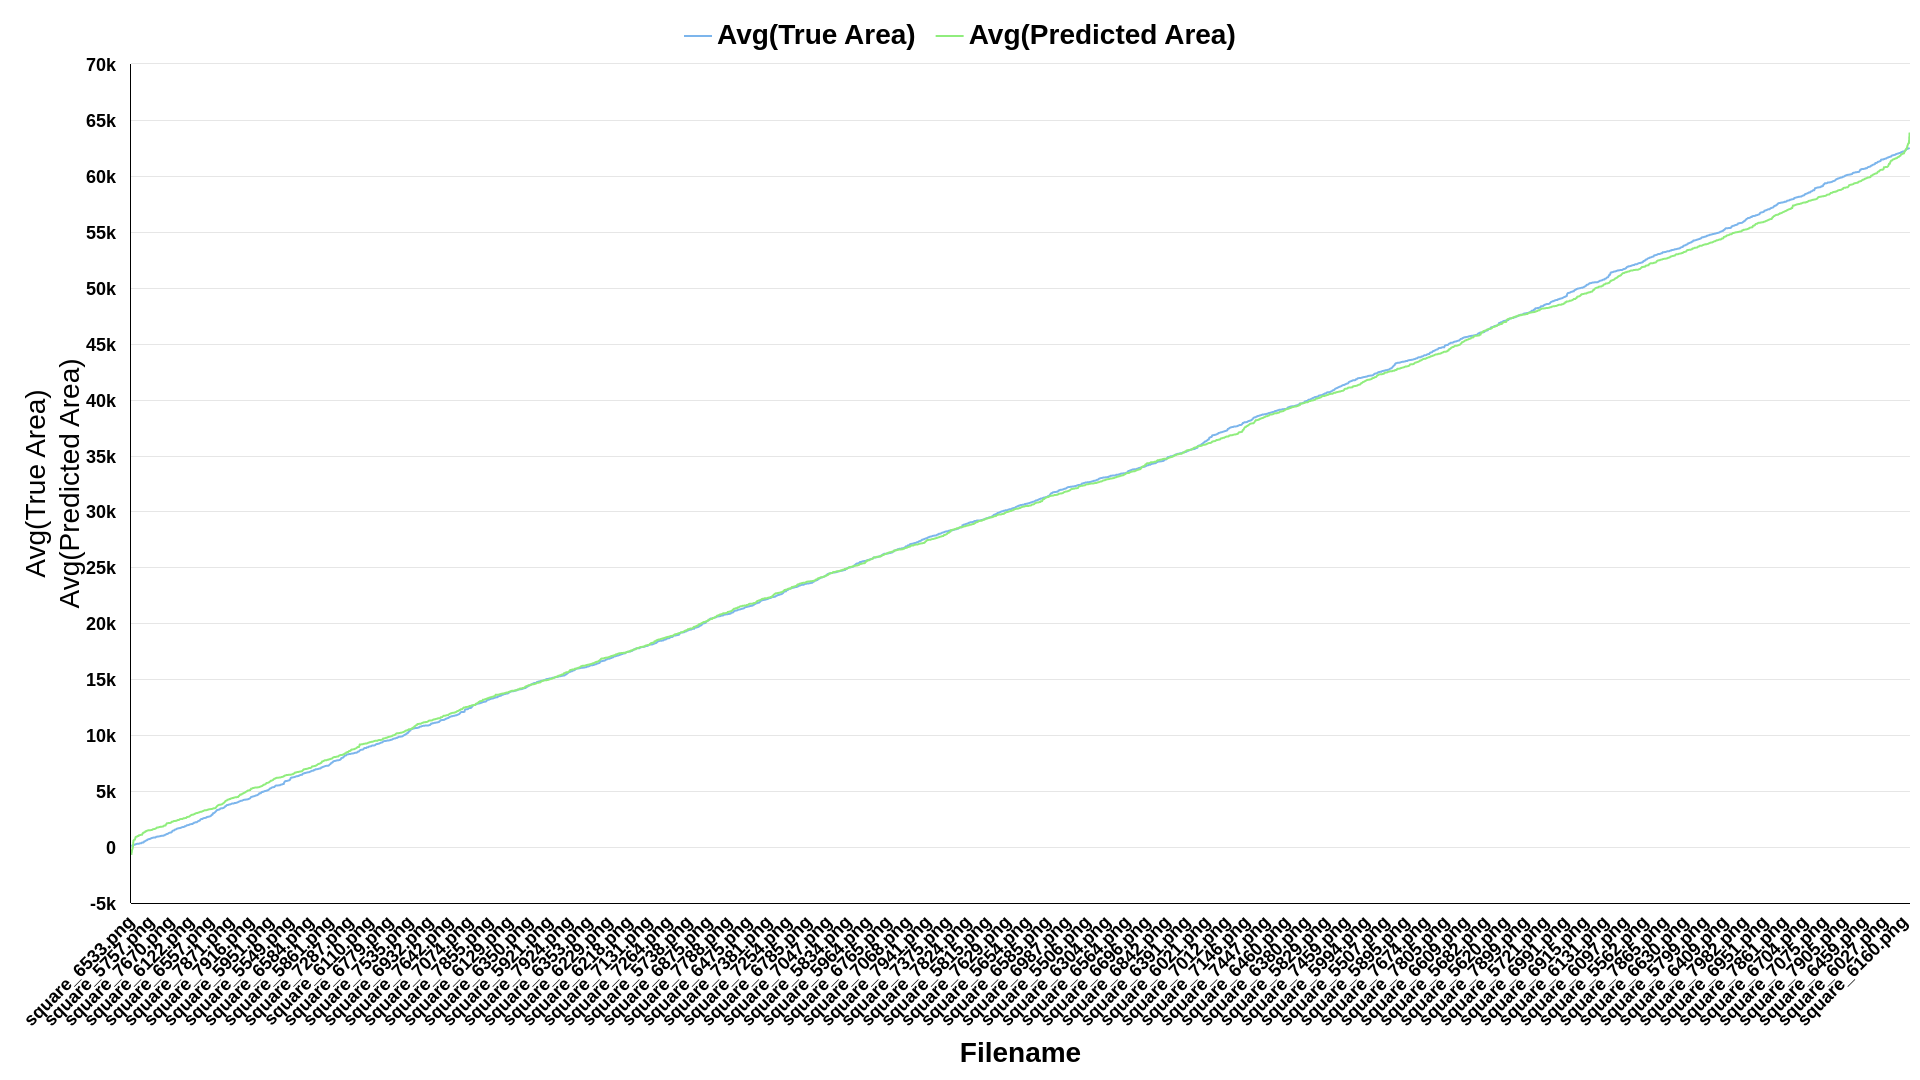
\includegraphics[width=1.0\linewidth]{imgs/Test_8/area_predict_true_line.png}
        \label{fig:enter-label}
    \end{figure}
    
       
        \begin{figure}[H]
        \centering
        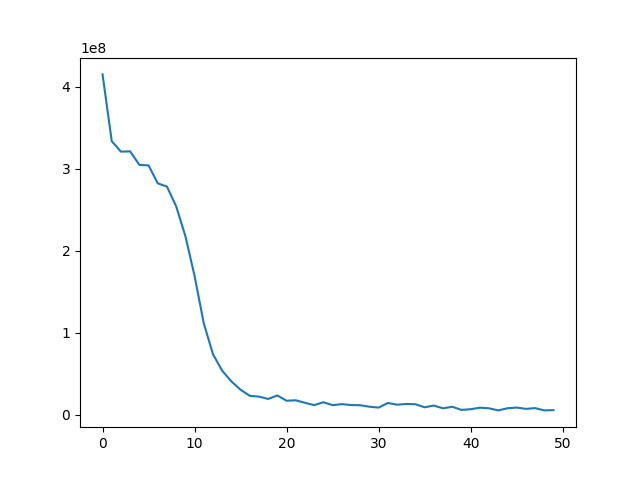
\includegraphics[width=1.0\linewidth]{imgs/Test_8/loss.png}
 
        \label{fig:enter-label}
    \end{figure}
    
       
        \begin{figure}[H]
        \centering
        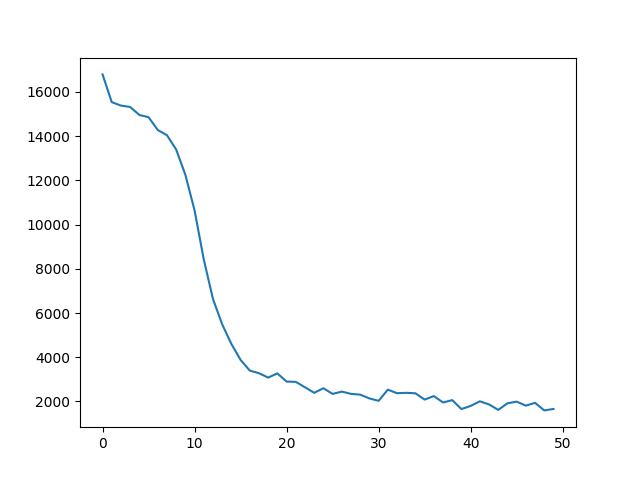
\includegraphics[width=1.0\linewidth]{imgs/Test_8/mae.png}
  
        \label{fig:enter-label}
    \end{figure}
    
    

\section{Teste 9}
\subsection{Objetivo}
    Classificar Imagens com quadrados, circulos e vazios. Ao seja, um problema de classificação não binário.
\subsection{Dataset}
    O Dataset é composto por 10998 imagens de treino e 4998 de teste. Composto por 3 classes: 
    \begin{itemize}
        \item Circulos 
        \item Quadrados
        \item Vazios
    \end{itemize}
    \begin{figure}[H]
        \centering
        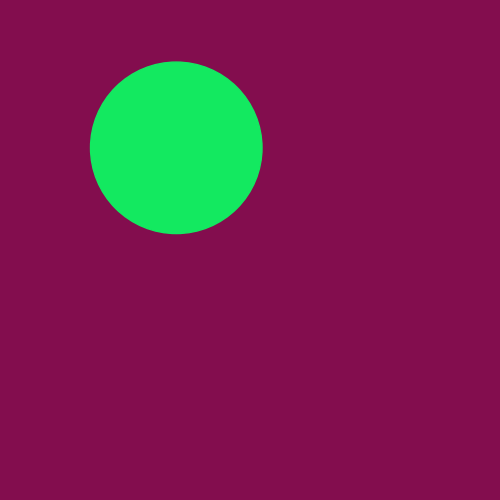
\includegraphics[width=0.25\linewidth]{imgs/Test_9/dataset_9/circles_4.png}
        
\includegraphics[width=0.25\linewidth]{imgs/Test_9/dataset_9/squares_4.png}
        
\includegraphics[width=0.25\linewidth]{imgs/Test_9/dataset_9/nones_3.png}
        \caption{Circlos, Quadrados e Vazios}
        \label{fig:enter-label}
    \end{figure}
    \begin{figure}[H]
        \centering
        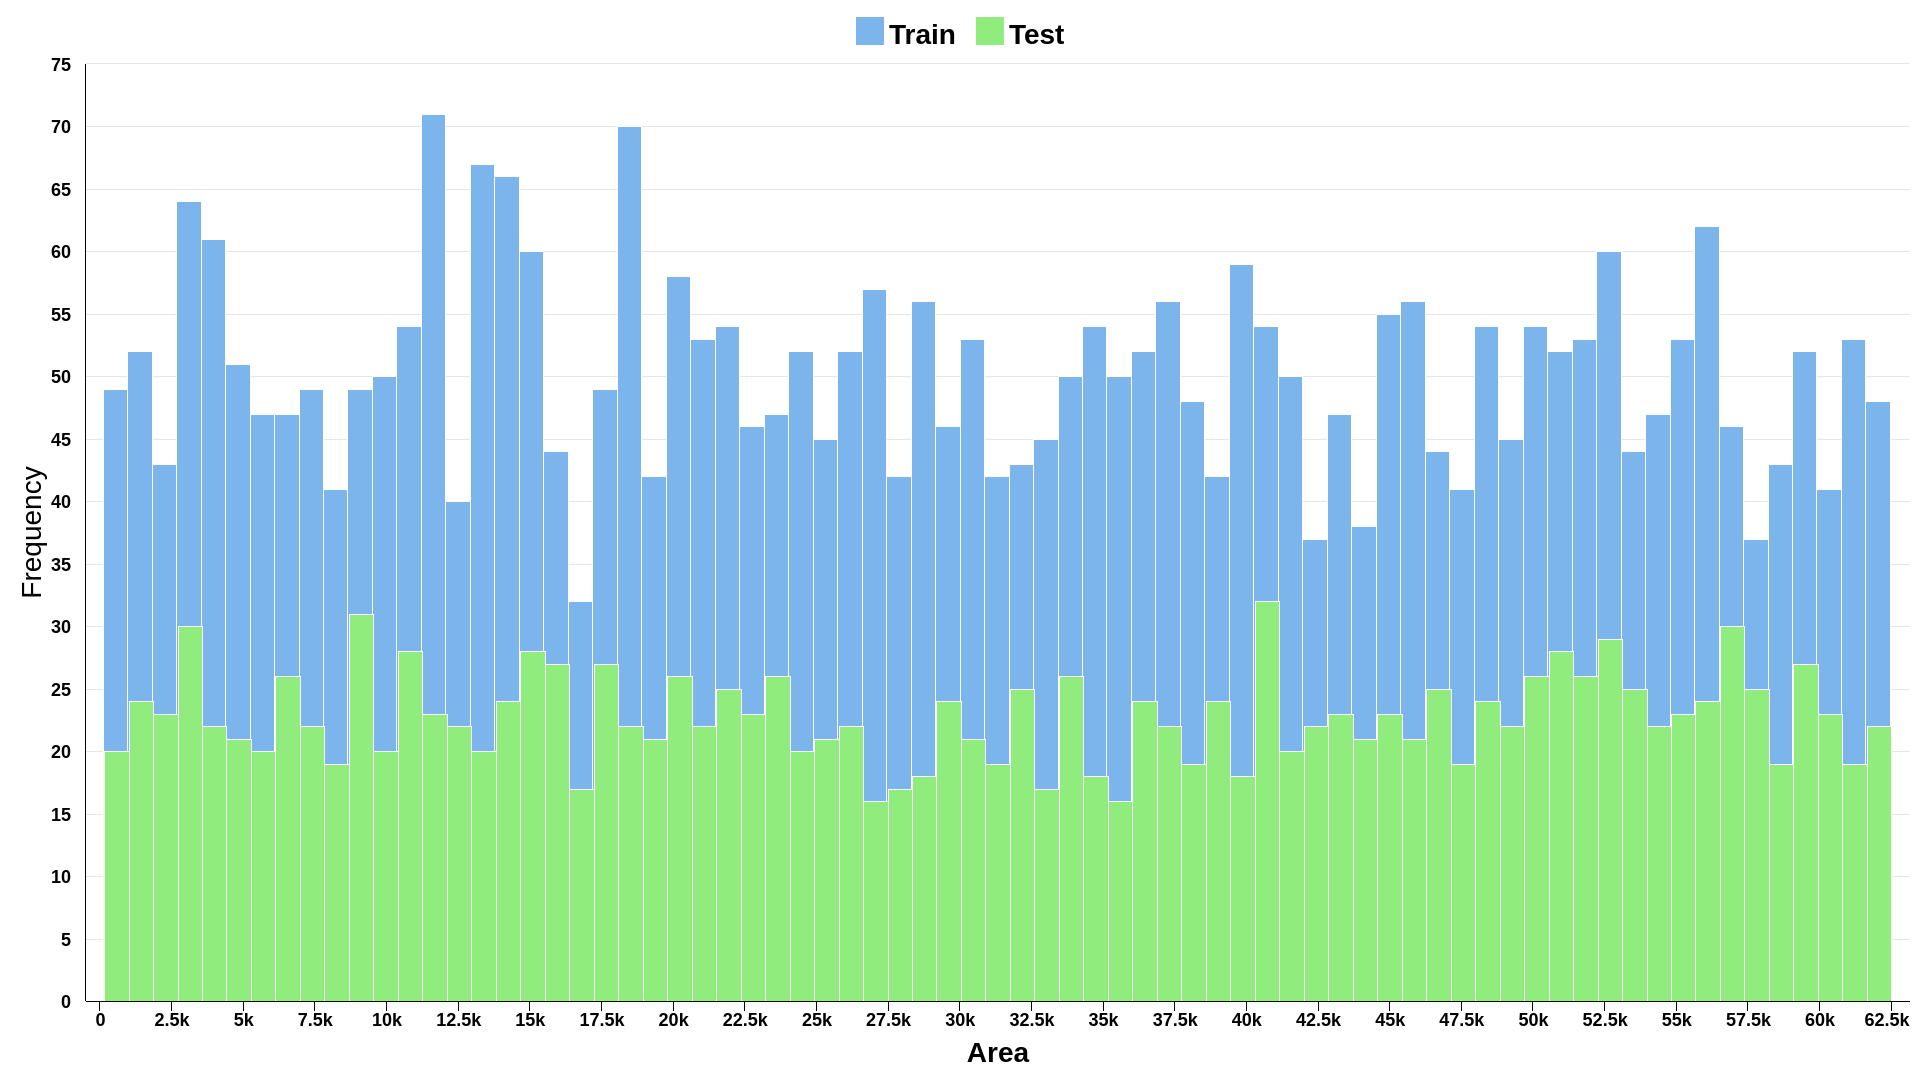
\includegraphics[width=1.0\linewidth]{imgs/Test_9/dataset_9/Squares_Area_Distribution_Hist.png}
        \caption{Distribuição da Área (Quadrados)}
        \label{fig:enter-label}
    \end{figure}
    \begin{figure}[H]
        \centering
        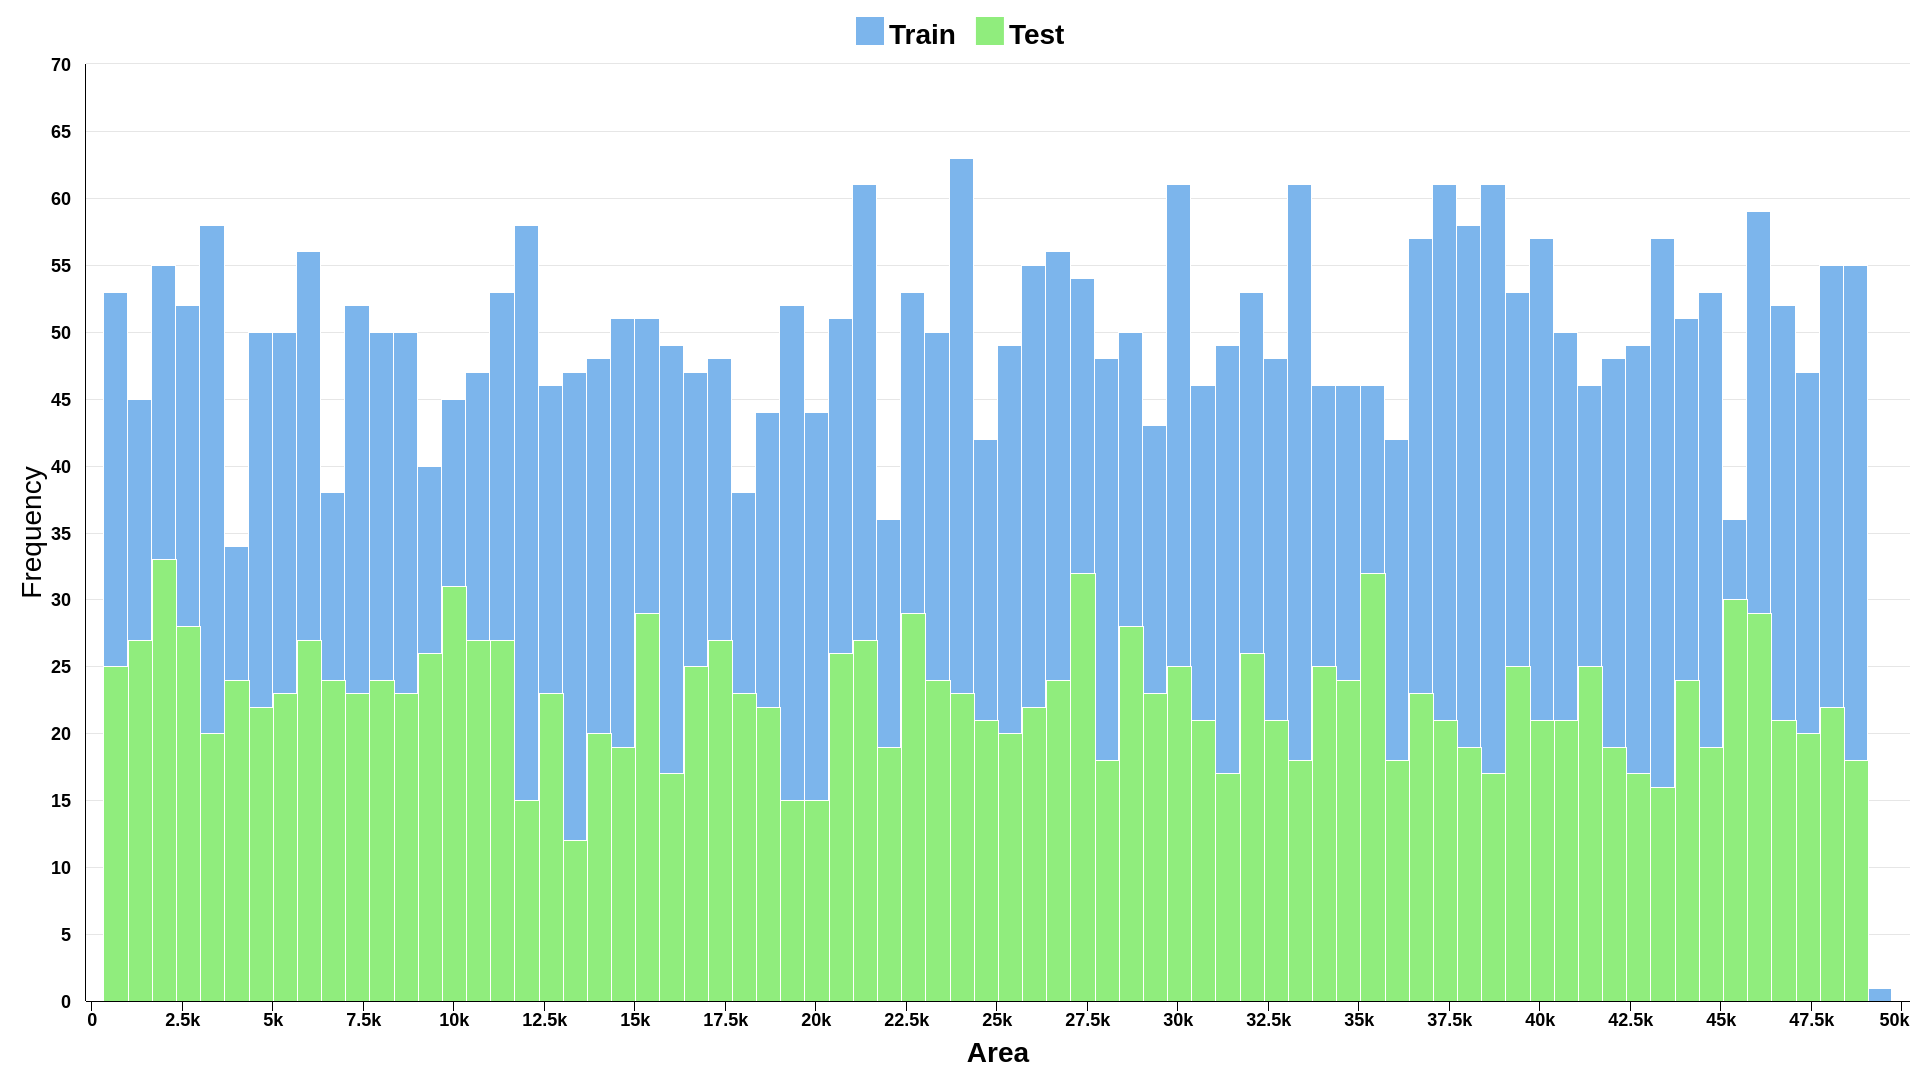
\includegraphics[width=1.0\linewidth]{imgs/Test_9/dataset_9/Circles_Area_Distribution_Hist.png}
        \caption{Distribuição da Área (Circulos)}
        \label{fig:enter-label}
    \end{figure}

\subsection{Treino}

\begin{figure}[H]
    \centering
    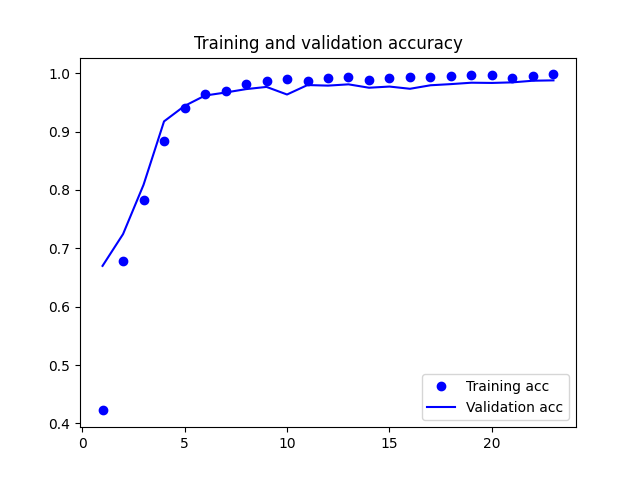
\includegraphics[width=\textwidth]{imgs/Test_9/train_test_acc.png}
    \caption{Acurácia de Validação e de Treino}
    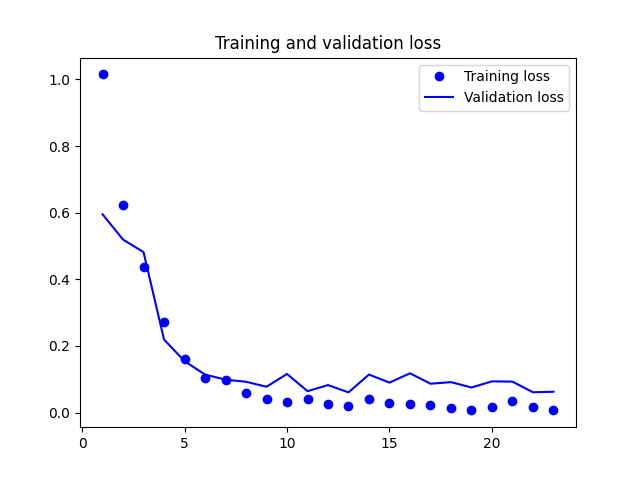
\includegraphics[width=\textwidth]{imgs/Test_9/train_test_loss.png}
    \caption{Perda de Validação e de Treino}
    \label{fig:sub2}
    Com as 23 épocas realizadas, conseguimos uma val acc de 0.9876, sendo que a melhor loss foi atingida na época 13.
\end{figure}

\subsection{Amostras Mal Classificadas}

No total foram mal classificadas 66 (1.32\% ) imagens, sendo 26 (39.39\%) delas circulos, 18 (27.27\%) quadrados e as restantes 22 (33.3\%) vazios. 

\subsection{Matriz de Confusão}

\begin{table}[H]
\centering
\begin{tabular}{l|c c c}
                 & Circulo & Quadrado & Vazio \\
\hline
Circulo          & 2405         & 22     & 1           \\
Quadrado         & 95           & 2330   & 1           \\
Vazio            & 95           & 2330   & 1           \\
\end{tabular}
\end{table}

\subsection{Análise}

\newpage

\section{Teste 10}
\subsection{Objetivo}
    Classificar Imagens com quadrados, circulos e vazios. Ao seja, um problema de classificação não binário.
\subsection{Dataset}
    O Dataset é composto por 10998 imagens de treino e 4998 de teste. Composto por 3 classes: 
    \begin{itemize}
        \item Circulos 
        \item Quadrados
        \item Triangulos
    \end{itemize}
    \begin{figure}[H]
        \centering
        
\includegraphics[width=0.25\linewidth]{imgs/Test_10/dataset_10/circles_9.png}
        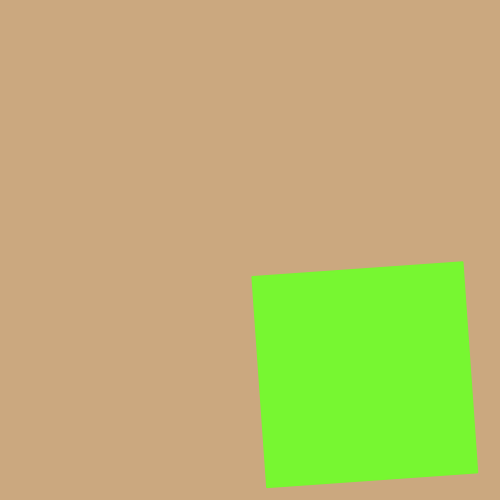
\includegraphics[width=0.25\linewidth]{imgs/Test_10/dataset_10/squares_9.png}
        \includegraphics[width=0.25\linewidth]{imgs/Test_10/dataset_910triangles_9.png}
        \caption{Circlos, Quadrados e Triangulos}
        \label{fig:enter-label}
    \end{figure}
    \begin{figure}[H]
        \centering
        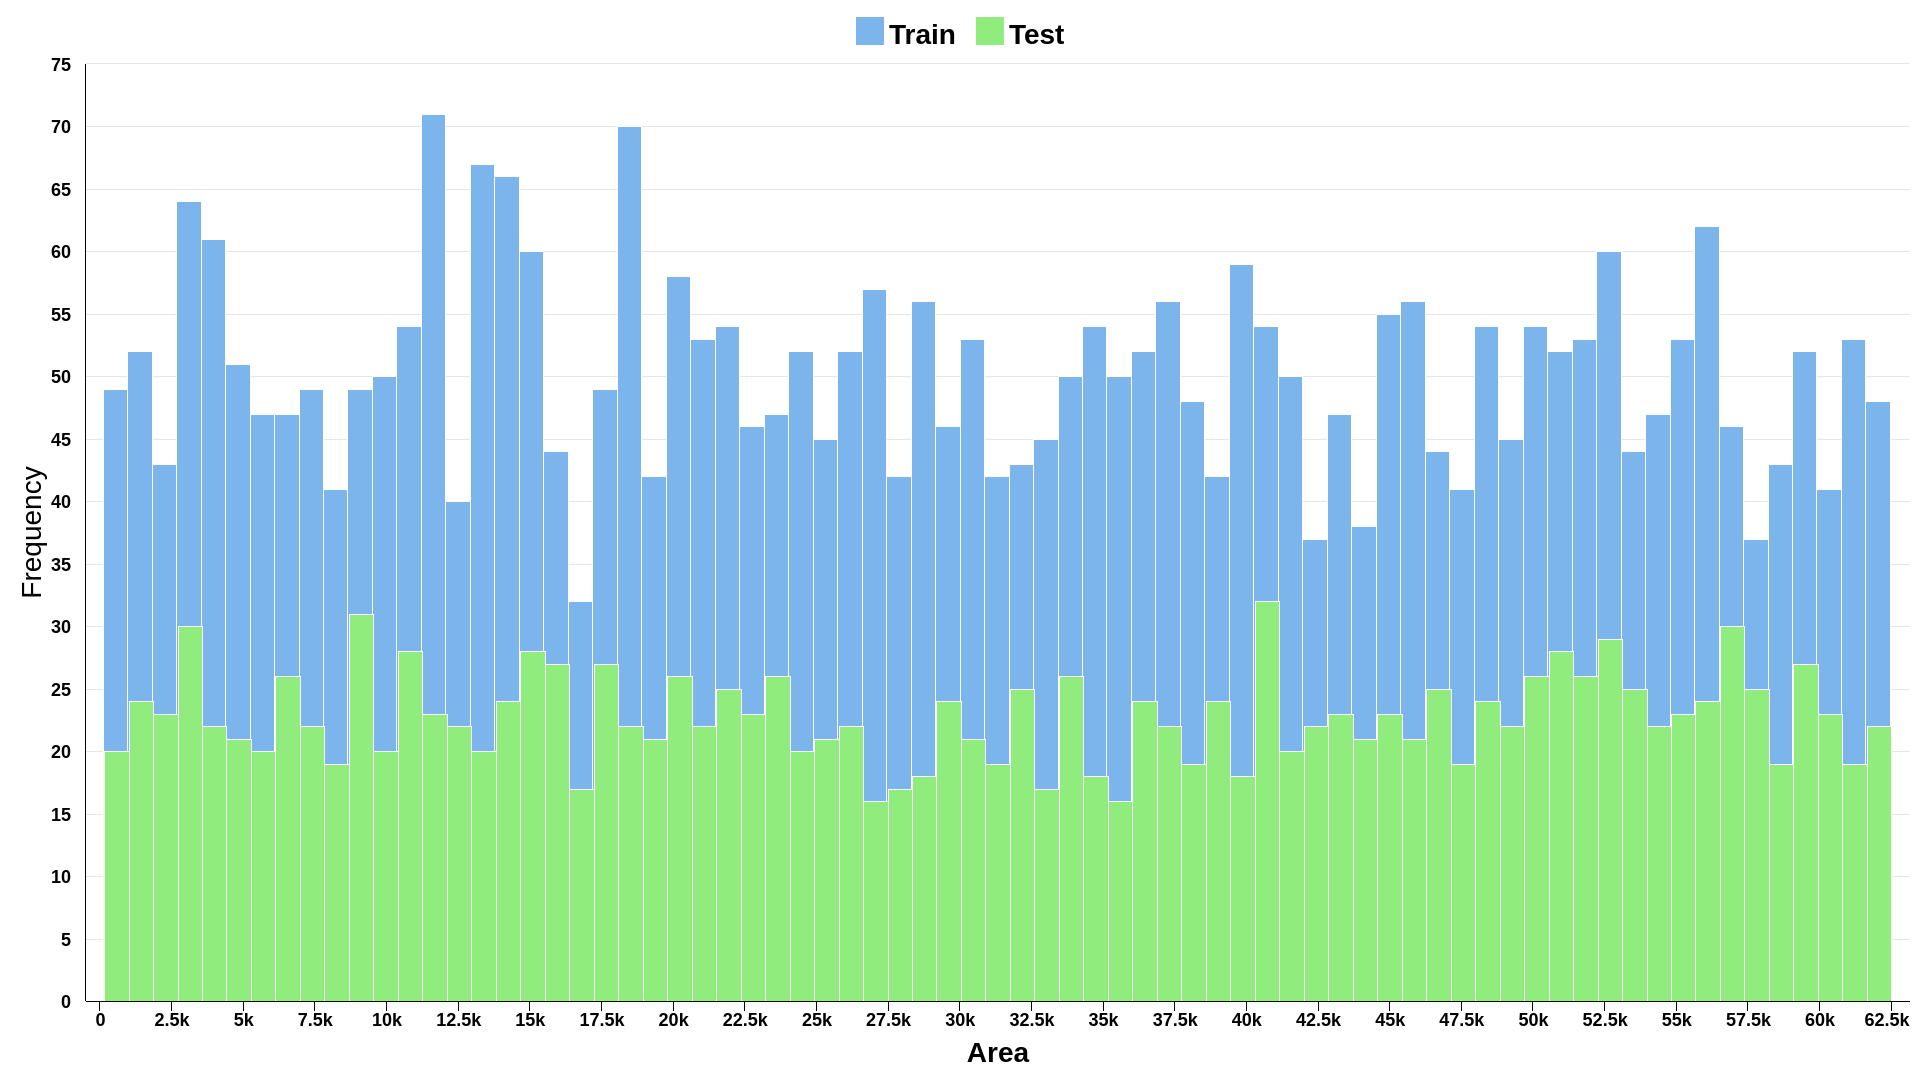
\includegraphics[width=1.0\linewidth]{imgs/Test_9/dataset_9/Squares_Area_Distribution_Hist.png}
        \caption{Distribuição da Área (Quadrados)}
        \label{fig:enter-label}
    \end{figure}
    \begin{figure}[H]
        \centering
        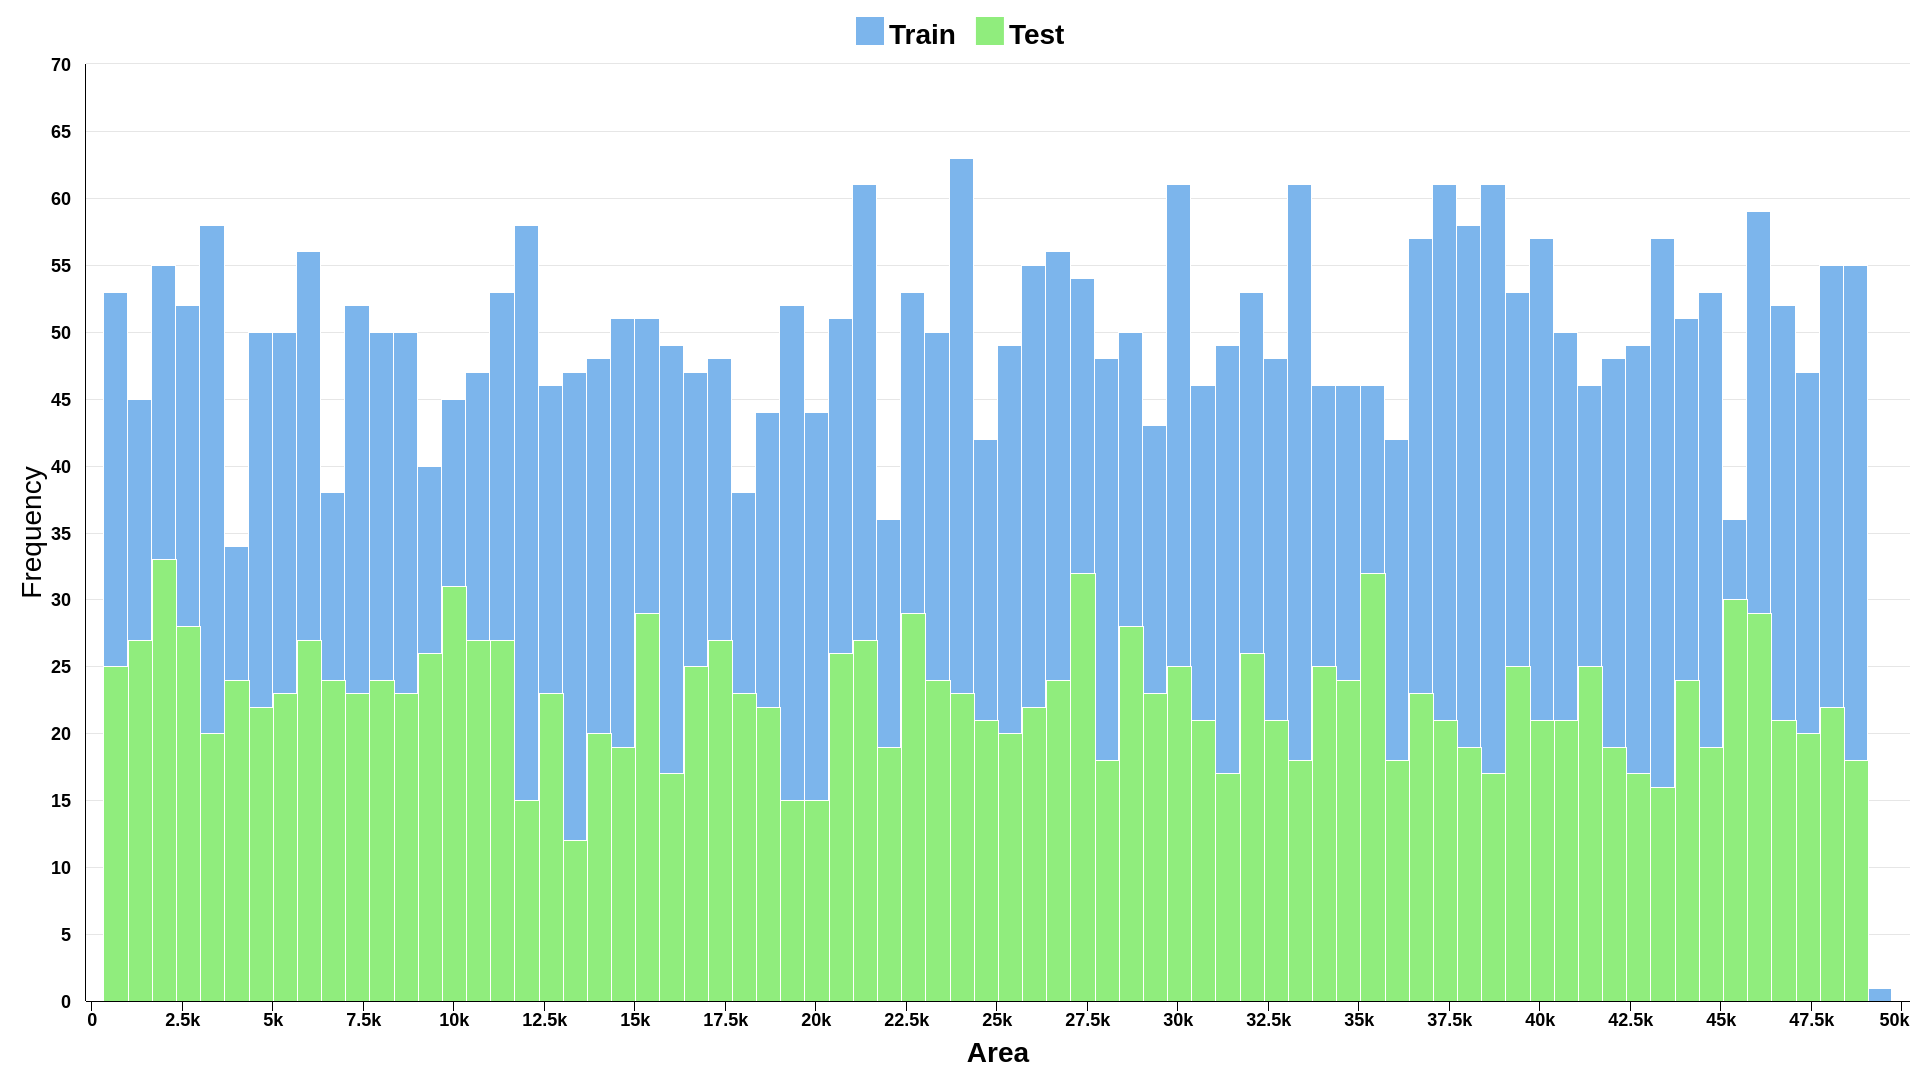
\includegraphics[width=1.0\linewidth]{imgs/Test_9/dataset_9/Circles_Area_Distribution_Hist.png}
        \caption{Distribuição da Área (Circulos)}
        \label{fig:enter-label}
    \end{figure}

\subsection{Treino}

\begin{figure}[H]
    \centering
    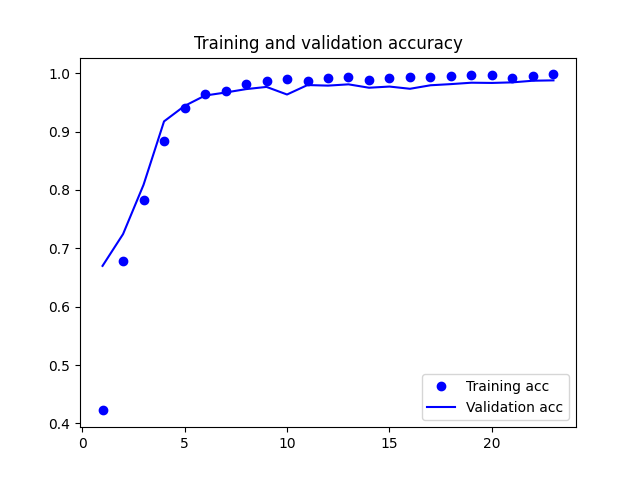
\includegraphics[width=\textwidth]{imgs/Test_9/train_test_acc.png}
    \caption{Acurácia de Validação e de Treino}
    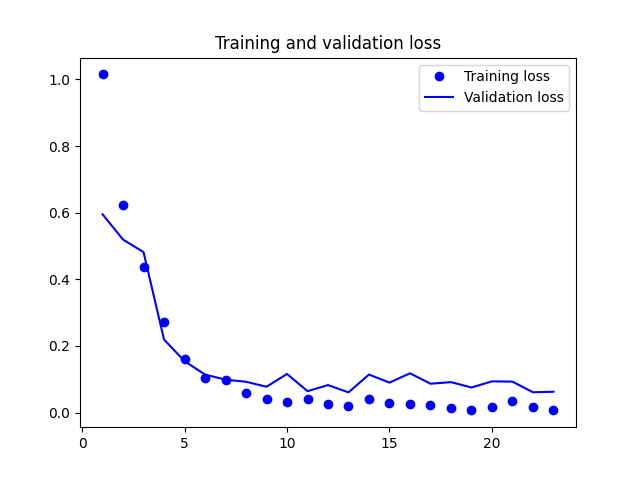
\includegraphics[width=\textwidth]{imgs/Test_9/train_test_loss.png}
    \caption{Perda de Validação e de Treino}
    \label{fig:sub2}
    Com as 23 épocas realizadas, conseguimos uma val acc de 0.9876, sendo que a melhor loss foi atingida na época 13.
\end{figure}

\subsection{Amostras Mal Classificadas}

No total foram mal classificadas 66 (1.32\% ) imagens, sendo 26 (39.39\%) delas circulos, 18 (27.27\%) quadrados e as restantes 22 (33.3\%) vazios. 

\subsection{Matriz de Confusão}

\begin{table}[H]
\centering
\begin{tabular}{l|c c c}
                 & Circulo & Quadrado & Vazio \\
\hline
Circulo          & 2405         & 22     & 1           \\
Quadrado         & 95           & 2330   & 1           \\
Vazio            & 95           & 2330   & 1           \\
\end{tabular}
\end{table}
\cleardoublepage\addtocontents{toc}{\protect\vspace{\beforebibskip}} % Place slightly below the rest of the document content in the table


%************************************************
\chapter{Conclusões}
\label{ch:conclusoes}
%************************************************


O uso do \LaTeXe permite-nos focar no essencial: o conteúdo, a formatação é tratada de forma automática.

Para mais informações sobre o \LaTeXe aconselha-se a consulta do
livro \emph{The Not So Short Introduction to \LaTeXe}~\cite{oetiker2000nss}.

Para a gestão de referências bibliográficas aconselha-se o JabRef. %\cite{jabref}.
 

\cleardoublepage%********************************************************************
% Bibliography
%*******************************************************
% work-around to have small caps also here in the headline
\manualmark
\markboth{\spacedlowsmallcaps{\bibname}}{\spacedlowsmallcaps{\bibname}} % work-around to have small caps also
\phantomsection 
\refstepcounter{dummy}
\addtocontents{toc}{\protect\vspace{\beforebibskip}} % to have the bib a bit from the rest in the toc
\addcontentsline{toc}{chapter}{\tocEntry{\bibname}}

\printbibliography
\label{app:bibliography} 


%********************************************************************
% Backmatter
%*******************************************************
\appendix

\cleardoublepage
\phantomsection 
\part*{Apêndices}

\cleardoublepage\addtocontents{toc}{\protect\vspace{\beforebibskip}} % Place slightly below the rest of the document content in the table

% If problems with the headers: get headings in appendix etc. right
\markboth{\spacedlowsmallcaps{Anexos}}{\spacedlowsmallcaps{Anexos}}

% Appendix A
\chapter{Apêncice A}

%----------------------------------------------------------------------------------------

\lipsum[13-14]

%----------------------------------------------------------------------------------------

\section{Appendix Section Test}
\lipsum[15]

\lipsum[16]

%----------------------------------------------------------------------------------------

\section{Another Appendix Section Test}
\lipsum[17]

\begin{table}
\myfloatalign
\begin{tabularx}{\textwidth}{Xll} \toprule
\tableheadline{labitur bonorum pri no} & \tableheadline{que vista}
& \tableheadline{human} \\ \midrule
fastidii ea ius & germano &  demonstratea \\
suscipit instructior & titulo & personas \\
\midrule
quaestio philosophia & facto & demonstrated \\
\bottomrule
\end{tabularx}
\caption[Autem usu id]{Autem usu id.}
\label{tab:moreexample}
\end{table}

\lipsum[18]





\cleardoublepage\addtocontents{toc}{\protect\vspace{\beforebibskip}} % Place slightly below the rest of the document content in the table

% Appendix X
\chapter{Apêncice B}
%----------------------------------------------------------------------------------------

% Content begins here


\lipsum[15]



\cleardoublepage%*******************************************************
% Declaration
%*******************************************************


\refstepcounter{dummy}
\addtocontents{toc}{\protect\vspace{\beforebibskip}} % to have the bib a bit from the rest in the toc
\addcontentsline{toc}{chapter}{\tocEntry{Declaração}}
\chapter*{Declaração}
\thispagestyle{empty}


% Declaro, sob compromisso de honra, que o trabalho apresentado nesta dissertação, com o título \textit{``\myTitle''}, é original e foi realizado por \myNameOne (\myNumber) sob orientação de \myProfOne.

\vspace{15 mm}

\noindent\textit{\myLocation, \myTime}
\bigskip

\begin{flushright}
    \begin{tabular}{m{8cm}}
        \\ \hline
        \centering\myNameOne \\
    \end{tabular}
\end{flushright}

% \vspace{5 mm}
% 
% \begin{flushright}
%     \begin{tabular}{m{8cm}}
%         \\ \hline
%         \centering\myNameTwo \\
%     \end{tabular}
% \end{flushright}




% 
% \begin{flushright}
%     \begin{tabular}{|m{10cm}}
%         \\ 
%         \centering  %\myName \\
%     \end{tabular}
% \end{flushright}
% 
% \vspace{5 mm}
% \begin{flushright}
%     \begin{tabular}{|m{10cm}}
%         \\ 
%         \centering  %\myName \\
%     \end{tabular}
% \end{flushright}
% 
% 

%********************************************************************
% Game Over: Restore, Restart, or Quit?
%*******************************************************
\end{document}
%********************************************************************
